% Survey — IJAR / Elsevier CAS format (cas-sc.cls)
% Compile: pdflatex main && bibtex main && pdflatex main && pdflatex main

\documentclass[a4paper,fleqn]{cas-sc}

\usepackage[numbers,sort&compress]{natbib}
\usepackage{doi}
\usepackage{float}
\usepackage{amsmath}
\usepackage{amsthm}
\usepackage{unicode-math}
\setmathfont{STIX Two Math}
\usepackage{booktabs}
\usepackage{multirow}
\usepackage{enumitem}
\usepackage{xcolor}
\usepackage[section]{placeins}
\usepackage{tikz}
\usetikzlibrary{arrows.meta,positioning,fit,backgrounds,shapes.geometric}
\emergencystretch=3em

% cas-sc renders corresponding-author mark as $\ast$ (U+2217), which
% Preview.app on macOS displays as "<" under XeLaTeX font embedding.
% Remap \ast to use the text-font asterisk (*) so the glyph is correct.
\AtBeginDocument{\renewcommand{\ast}{\text{*}}}

\hypersetup{colorlinks=true,allcolors=blue,
  pdftitle={When Modern Mathematics Meets Granular Computing},
  pdfauthor={Thanh Dai Tran and Long Giang Nguyen},
  pdfsubject={Granular computing; rough sets; feature selection; survey},
  pdfkeywords={Granular computing; Neighbourhood rough sets; Feature selection;
               Persistent homology; Negative results; Benchmark methodology}
}

\pdfstringdefDisableCommands{%
  \def\corref#1{}%
  \def\cnotenum#1{}%
  \def\fnref#1{}%
}

% ── Notation shortcuts ────────────────────────────────────────────────────────
\newcommand{\U}{\mathcal{U}}
\newcommand{\C}{\mathcal{C}}
\newcommand{\POS}{\mathrm{POS}}
\newcommand{\LOW}{\underline{\mathrm{apr}}}
\newcommand{\UPP}{\overline{\mathrm{apr}}}
\newcommand{\RED}{\mathrm{RED}}
\newcommand{\DEP}{\gamma}
\newcommand{\NB}[1]{\delta_{#1}}

\begin{document}
\let\WriteBookmarks\relax
\def\floatpagepagefraction{.8}
\def\textpagefraction{.1}
\setlength{\textfloatsep}{10pt plus 2pt minus 2pt}
\setlength{\floatsep}{8pt plus 2pt minus 2pt}
\setlength{\intextsep}{8pt plus 2pt minus 2pt}
\setlength{\dbltextfloatsep}{10pt plus 2pt minus 2pt}
\setlength{\dblfloatsep}{8pt plus 2pt minus 2pt}

\shorttitle{Modern Mathematics Meets Granular Computing}
\shortauthors{T.D.~Tran and L.G.~Nguyen}

\title[mode=title]{When Modern Mathematics Meets Granular Computing:
A Critical Survey of What Works, What Fails, and Why}

\author[1]{Thanh Dai Tran}
\cormark[1]
\corref{cor1}
\ead{ttdaiuneti@gmail.com}
\credit{Conceptualization, Methodology, Software, Validation, Formal analysis,
        Investigation, Writing -- original draft, Writing -- review \& editing}

\author[2]{Long Giang Nguyen}
\ead{nlgiang@ioti.vn}
\credit{Conceptualization, Methodology, Writing -- review \& editing,
        Project administration}

\affiliation[1]{organization={University of Economics and Technology for
                Industries (UNETI)},
            addressline={456 Minh Khai, Hai Ba Trung District},
            city={Hanoi},
            postcode={100000},
            country={Vietnam}}

\affiliation[2]{organization={Institute of Information Technology,
                Vietnam Academy of Science and Technology (VAST)},
            addressline={18 Hoang Quoc Viet, Cau Giay District},
            city={Hanoi},
            postcode={100000},
            country={Vietnam}}

\cortext[cor1]{Corresponding author.}

\begin{abstract}
Granular computing has spent two decades developing a principled toolkit
for handling uncertainty in decision tables: equivalence and neighbourhood
granules, lower and upper approximations, positive regions, and attribute
reducts.  A recent wave of papers imports frameworks from modern mathematics
and machine learning---persistent homology, fuzzy topology, conformal
prediction, weak supervision---into this core machinery.  We present a
critical survey of this wave, organised around a single thesis: when a
modern framework is imported into granular computing's core pipeline, the
resulting quantity tends either (a) to reduce to an already-known granular
quantity, (b) to be dominated by geometry of the feature distribution that is
orthogonal to the decision problem---of which measurement scale is the
special case our bound captures---or (c) to win only where the evaluation
is aligned with its own objective---either algebraically, or through a free
parameter of the metric that the analyst sets.  These three failure patterns explain why the volume of
``GrC + X'' papers has grown rapidly while progress has been slower.
Our survey is unusual in that the thesis is backed by our own negative-result
experiments: $4{,}975$ attribute-importance measurements, $30{,}100$
downstream classification records, and $995$ structure-preservation
measurements across ten UCI datasets, all released per-fold for
reproducibility.  A further ablation shows that the one metric on which the
imported method appears to lead reverses its verdict when that metric's own
neighbourhood parameter is varied over unchanged feature subsets---an
instance of the evaluation problem the survey documents.  Beyond cataloguing the state of the art across four axes
(granule geometry, topological formalisms, computational efficiency,
sufficiency and limits), we document a methodological pattern in the field:
comparisons on 3-NN/SVM with default hyperparameters on small UCI benchmarks
often cannot detect differences beyond measurement noise, yet results are
reported as improvements without significance testing.  Coding 22 papers at
full text---13 of them a majority of our granule-geometry corpus---we find
none that reports an all-features baseline, dispersion, a significance test
and a hyperparameter ablation together; the per-paper coding is released with
a supporting quotation for every judgement.
\end{abstract}

\begin{highlights}
\item Three recurring failure patterns (reduction, label-orthogonal geometry,
      self-optimising evaluation) explain the gap between publication volume
      and progress in the GrC literature.
\item A persistence-based attribute importance score is shown to be
      uncorrelated with neighbourhood-based discriminability
      (Fisher-$z$ $\bar\rho = -0.060$, 95\% CI $[-0.21,\,+0.09]$)
      and statistically indistinguishable from a null baseline.
\item $4{,}975$ importance measurements and $30{,}100$ classification records
      are released per-fold for reproducibility.
\item A six-point minimum reporting standard is proposed for GrC
      feature-selection experiments.
\item Nine open problems are identified across four axes,
      with explicit barriers and requirements for a solution.
\end{highlights}

\begin{keywords}
Granular computing \sep Neighbourhood rough sets \sep Feature selection \sep
Attribute reduction \sep Persistent homology \sep Negative results \sep
Benchmark methodology
\end{keywords}

\maketitle

% ── Theorem-like environments (after \maketitle, as required by cas-sc) ───────
\newtheorem{theorem}{Theorem}
\newtheorem{proposition}{Proposition}
\newtheorem{corollary}{Corollary}
\newtheorem{lemma}{Lemma}
\theoremstyle{definition}
\newtheorem{definition}{Definition}
\newtheorem{remark}{Remark}
\newtheorem{example}{Example}

% ── Body sections ─────────────────────────────────────────────────────────────
\section{Introduction}
\label{sec:intro}

Granular computing (GrC) has spent four decades building a principled
toolkit for decision-making under incomplete information.  The conceptual
roots lie in Zadeh's information granularity~\cite{Zadeh1979granularity},
Lin's neighbourhood systems~\cite{Lin1998neighborhood}, and Pedrycz's
programmatic formulation of granular
computing~\cite{Pedrycz2001GrC}.  Starting from
Pawlak's rough sets~\cite{Pawlak1982}, the field has produced a rich theory
of granules (equivalence classes, neighbourhood balls, covering sets),
approximation operators (lower, upper, boundary), and knowledge reduction
(attribute reduct, discernibility).  Neighbourhood rough sets
(NRS)~\cite{Hu2008NRS} extended this framework to continuous data;
granular ball NRS (GBNRS)~\cite{Xia2020GBNRS} further replaced the
fixed-radius ball with a purity-controlled adaptive granule, accumulating
259 citations since 2020 (retrieved September 2025).

The past decade has seen a wave of papers importing frameworks from modern
mathematics and machine learning into this core pipeline.  Persistent
homology offers a multi-scale topological summary of a point cloud.
Fuzzy topology and Alexandrov preorders generalise the equivalence
relation.  Conformal prediction and weak supervision address label
uncertainty.  These are powerful tools; the GrC community's interest in
them is legitimate.

\paragraph{The thesis of this survey.}
Our central finding, supported by a systematic literature review and by
original negative-result experiments, is the following.

\begin{quote}
When a modern mathematical or ML framework is imported into GrC's core
pipeline (neighbourhood granule $\to$ approximation $\to$ reduct), the
resulting quantity tends to either (A) reduce to an already-known
granular quantity, (B) be dominated by geometry of the feature distribution
that is orthogonal to the decision problem, or (C) succeed only where the
evaluation
is aligned with its own objective---whether algebraically, or through a free
parameter of the metric.
\end{quote}

We call these \emph{Pattern A}, \emph{Pattern B}, and \emph{Pattern C}.
Figure~\ref{fig:patterns} locates each pattern in the GrC pipeline and
gives a concrete instantiation; Sections~\ref{sec:patA}--\ref{sec:patC}
provide experimental verification of each.

\begin{figure*}[pos=!htbp]
\centering
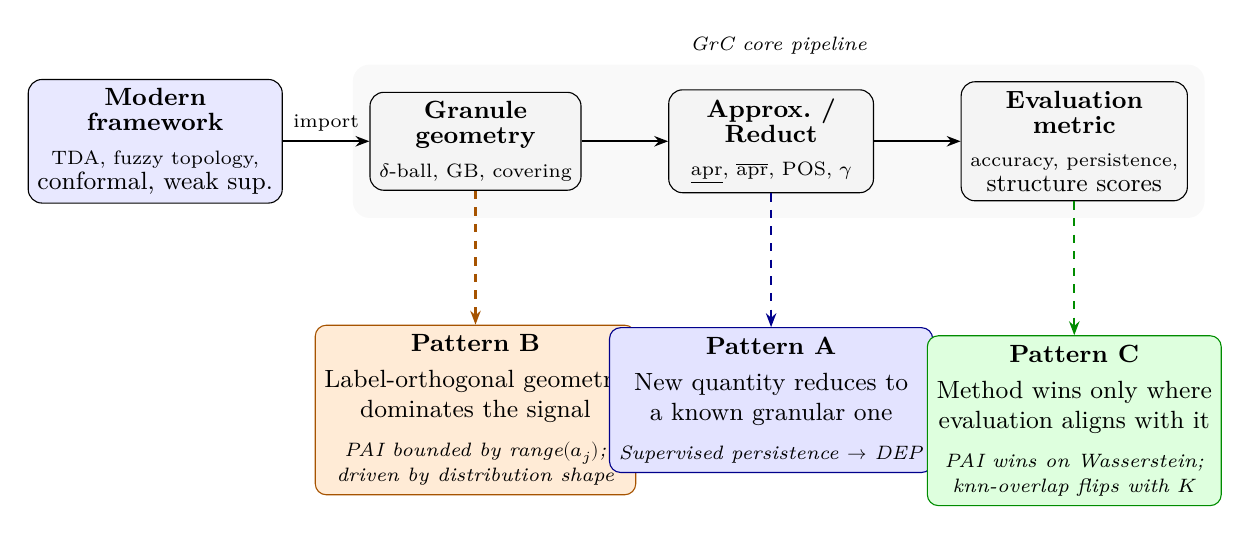
\begin{tikzpicture}[
  %% style definitions
  stage/.style  = {draw, rounded corners=5pt, fill=gray!9,
                   minimum width=2.6cm, minimum height=1.1cm,
                   align=center, font=\small},
  import/.style = {draw, rounded corners=5pt, fill=blue!9,
                   minimum width=2.6cm, minimum height=1.1cm,
                   align=center, font=\small},
  patbox/.style = {draw, rounded corners=4pt,
                   minimum width=3.0cm, minimum height=1.55cm,
                   align=center, font=\small},
  patA/.style   = {patbox, fill=blue!11,   draw=blue!55!black},
  patB/.style   = {patbox, fill=orange!16, draw=orange!65!black},
  patC/.style   = {patbox, fill=green!13,  draw=green!55!black},
  arr/.style    = {-{Stealth[length=5pt]}, thick},
  darr/.style   = {-{Stealth[length=5pt]}, thick, dashed},
  lbl/.style    = {font=\scriptsize, midway, above},
]

%% ── Pipeline (top row) ───────────────────────────────────────────────────────
\node[import] (fw)     at (0,0)
  {\textbf{Modern}\\[-2pt]\textbf{framework}\\[1pt]
   \scriptsize TDA, fuzzy topology,\\[-2pt]conformal, weak sup.};

\node[stage, right=1.1cm of fw]   (gran)
  {\textbf{Granule}\\[-2pt]\textbf{geometry}\\[1pt]
   \scriptsize $\delta$-ball, GB, covering};

\node[stage, right=1.1cm of gran] (approx)
  {\textbf{Approx.\ /}\\[-2pt]\textbf{Reduct}\\[1pt]
   \scriptsize $\underline{\mathrm{apr}}$, $\overline{\mathrm{apr}}$, $\mathrm{POS}$, $\gamma$};

\node[stage, right=1.1cm of approx] (eval)
  {\textbf{Evaluation}\\[-2pt]\textbf{metric}\\[1pt]
   \scriptsize accuracy, persistence,\\[-2pt]structure scores};

%% ── Pipeline arrows ──────────────────────────────────────────────────────────
\draw[arr] (fw)     -- node[lbl]{import} (gran);
\draw[arr] (gran)   --                   (approx);
\draw[arr] (approx) --                   (eval);

%% ── Pattern boxes (bottom row) ───────────────────────────────────────────────
\node[patB, below=1.7cm of gran]
  (pB) {\textbf{Pattern B}\\[2pt]
        Label-orthogonal geometry\\dominates the signal\\[3pt]
        \textit{\scriptsize PAI bounded by range$(a_j)$;}\\[-2pt]
        \textit{\scriptsize driven by distribution shape}};

\node[patA, below=1.7cm of approx]
  (pA) {\textbf{Pattern A}\\[2pt]
        New quantity reduces to\\a known granular one\\[3pt]
        \textit{\scriptsize Supervised persistence $\to$ DEP}};

\node[patC, below=1.7cm of eval]
  (pC) {\textbf{Pattern C}\\[2pt]
        Method wins only where\\evaluation aligns with it\\[3pt]
        \textit{\scriptsize PAI wins on Wasserstein;}\\[-2pt]
        \textit{\scriptsize knn-overlap flips with $K$}};

%% ── Downward dashed arrows ────────────────────────────────────────────────────
\draw[darr, orange!65!black] (gran.south)   -- (pB.north);
\draw[darr, blue!55!black]   (approx.south) -- (pA.north);
\draw[darr, green!55!black]  (eval.south)   -- (pC.north);

%% ── Background shading for GrC pipeline ─────────────────────────────────────
\begin{scope}[on background layer]
  \node[fill=gray!5, rounded corners=6pt,
        fit=(gran)(approx)(eval),
        inner sep=6pt, label={[font=\scriptsize\itshape]above:GrC core pipeline}] {};
\end{scope}

\end{tikzpicture}
\caption{Three structural failure patterns arising when a modern mathematical
or ML framework is imported into GrC's core pipeline.
\textbf{Pattern~A}: the new quantity reduces algebraically to a known granular
measure (\S\ref{sec:patA}).
\textbf{Pattern~B}: the importance signal is dominated by label-orthogonal
properties of the feature's distribution---measurement scale being the
special case a stability bound captures (\S\ref{sec:patB}).
\textbf{Pattern~C}: the method wins only where evaluation aligns with its own
objective---algebraically, or via a metric parameter the analyst chooses---and
not on criteria that are robust to that choice (\S\ref{sec:patC}).
Each pattern is diagnosable before implementation (Section~\ref{sec:checklist}).}
\label{fig:patterns}
\end{figure*}

This is not a pessimistic thesis.  Patterns~A--C are diagnostic, not
prohibitive.  They can be checked before implementation
(Section~\ref{sec:checklist}), saving months of wasted work.  And the
nine open problems in Section~\ref{sec:open} are open precisely
because they cannot be solved by a naive import of an existing framework.

\paragraph{Positioning.}
Most surveys in the GrC/rough-set space are taxonomic: they organise
papers by method type and report improvements in mean accuracy.
Yuan et al.~\cite{Yuan2021survey} survey fuzzy rough set attribute reduction
(126 citations); Kuzudisli et al.~\cite{Kuzudisli2023review} survey
grouping-based feature selection (69 citations); Santos et
al.~\cite{Santos2022overlap} survey class overlap complexity (93 citations);
Liu et al.~\cite{Liu2026survey} survey rough feature
selection algorithms across accelerated, incremental, weakly-supervised, and
multi-granularity variants---the broadest scope among these four surveys,
covering several directions that overlap with our Axes~1 and~3.
Liu et al.\ catalogue methods; we diagnose \emph{failure modes} when
external frameworks enter the pipeline, and back the diagnosis with
negative-result experiments that their survey does not attempt.
These are valuable contributions.
Table~\ref{tab:survey_compare} summarises the key differences.

\begin{table}[pos=!htbp]
\caption{Comparison with prior surveys in the GrC / rough-set feature-selection
area.  ``Expt.'' = original experiments; ``Fail.\ diag.'' = failure-pattern
diagnosis; ``Data rel.'' = raw data released.}
\label{tab:survey_compare}
\centering\small
\setlength\tabcolsep{3pt}
\begin{tabular}{p{3.2cm}cccccc}
\toprule
Survey & Scope & Period & \#Papers & Expt. & Fail.\ diag. & Data rel. \\
\midrule
Yuan et al.~\cite{Yuan2021survey}
  & Fuzzy RS reduction & 2000--2020 & 96 & Yes & No & No \\
Kuzudisli et al.~\cite{Kuzudisli2023review}
  & Grouping-based FS & 2010--2022 & 82 & No & No & No \\
Santos et al.~\cite{Santos2022overlap}
  & Class overlap & 2000--2021 & 120 & No & No & No \\
Liu et al.~\cite{Liu2026survey}
  & Rough FS algorithms & 2005--2025 & 150+ & No & No & No \\
\textbf{This survey}
  & GrC + modern math. & 2000--2025 & 52 & Yes & Yes & Yes \\
\bottomrule
\end{tabular}
\end{table}

The closest precursor to our own work is Yuan et al.~\cite{Yuan2021survey},
published in Applied Soft Computing, which surveys fuzzy
rough set attribute reduction methods via comparative experiments on 12 UCI
datasets.  That paper's scope and ours are complementary rather than
overlapping.  Yuan et al.\ cover fuzzy rough set methods---a specific
formal variant of the rough set framework---and evaluate them on mean accuracy
benchmarks.  Our survey covers \emph{what happens when modern mathematical
frameworks} (topology, persistent homology, conformal prediction, weak
supervision) are imported into the broader granular computing pipeline; it
does not survey fuzzy rough sets as a family.  Methodologically, we add what
Yuan et al.\ did not: a falsifiable thesis about structural failure modes,
negative-result experimental evidence, and a critique of the benchmark
methodology used across the community (including papers like those surveyed
in Yuan et al.).

Across these surveys, our work stands apart in being diagnostic rather than
cataloguing: we argue that a specific structural dynamic limits the GrC+X
literature, we provide original experimental evidence for it, and we show
with data---not opinion---that the field's dominant evaluation protocol is
often insensitive to the differences it purports to detect.  Concretely,
this survey contributes:

\begin{enumerate}
  \item \textbf{A falsifiable thesis} (Patterns~A--C) about how imported
        frameworks fail, with an explicit refutation condition for each
        (Sections~\ref{sec:failure} and~\ref{sec:open}).
  \item \textbf{A taxonomy of the topological literature} into two
        branches that our corpus shows to be unconnected, with the
        conditions under which bridging them avoids Pattern~A
        (Section~\ref{sec:topology}).
  \item \textbf{A saturation assessment of granule geometry}
        (Table~\ref{tab:granule_tax}): the natural deformations of the
        neighbourhood ball have each been taken (Section~\ref{sec:geometry}).
  \item \textbf{Original negative-result experiments}---$4{,}975$
        importance measurements and $30{,}100$ classification records,
        released per fold---documenting where a designed-to-succeed method
        fails and why, with a bound (Theorem~\ref{thm:pai_bound}) that
        explains the mechanism (Section~\ref{sec:patB}).
  \item \textbf{A data-driven methodology critique} showing that on seven of
        ten standard benchmarks the best reduct is not statistically
        separable from using every feature, and that across 22 papers read at
        full text---13 of them, a majority of our Axis-1 corpus---not one
        reports all four of an all-features baseline, dispersion, a
        significance test and a hyperparameter ablation, with the per-paper
        coding released for audit (Section~\ref{sec:methodology}).
  \item \textbf{A diagnostic checklist and a six-point reporting standard},
        applicable before implementation (Sections~\ref{sec:checklist}
        and~\ref{sec:standard}), together with nine open problems and the
        barrier that keeps each open (Section~\ref{sec:open}).
\end{enumerate}

Two audiences are addressed directly: the granular-computing researcher
weighing whether to import a modern framework, who should read
Sections~\ref{sec:failure} and~\ref{sec:open} first; and the reviewer or
editor asking why so many GrC feature-selection papers report improvements
that do not replicate, for whom Section~\ref{sec:methodology} is the
relevant part.

\paragraph{Scope.}
The four survey axes are not mutually exclusive: GBNRS appears in both
Axis~1 (geometry) and Axis~3 (efficiency), and three-way decision spans
Axis~1 and Axis~4.  Papers spanning multiple axes are catalogued under
their primary contribution.
We cover the period 2000--2025 with emphasis on 2018--2025, focusing on
feature selection and attribute reduction.  Three-way decision (3WD) and
multi-criteria decision analysis are included where they interact directly
with granule geometry or constitute an actively growing extension of the
core pipeline (Sections~\ref{sec:geo_emerging} and~\ref{sec:trends});
they are not surveyed as standalone paradigms.  We include 52 papers that
passed our inclusion criteria (Appendix~\ref{app:search}); a further 11
background and foundational references are cited as needed.

\paragraph{Organisation.}
Figure~\ref{fig:activity} illustrates the publication-year distribution of
surveyed papers across the four axes: Axis~1 (Granule Geometry) dominates
recent output, while Axes~3 and~4 remain sparse---a pattern that motivates
both the saturation argument (Section~\ref{sec:saturation}) and the open
problems (Section~\ref{sec:open}).
Section~\ref{sec:background} fixes notation.
Sections~\ref{sec:geometry}--\ref{sec:sufficiency} survey the four axes.
Section~\ref{sec:failure} presents the three failure patterns with
experimental evidence.  Section~\ref{sec:methodology} critiques the
field's evaluation practices.  Section~\ref{sec:trends} analyses three
research trends showing sustained momentum---incremental feature selection,
three-way decision integration, and neural-augmented granular
computing---and identifies the conditions under which each avoids the
failure patterns.  Section~\ref{sec:open} lists nine open problems.
Section~\ref{sec:conclusion} concludes.
Figure~\ref{fig:roadmap} provides a bird's-eye view of the survey
structure and the connections between sections.

\begin{figure*}[pos=!htbp]
\centering
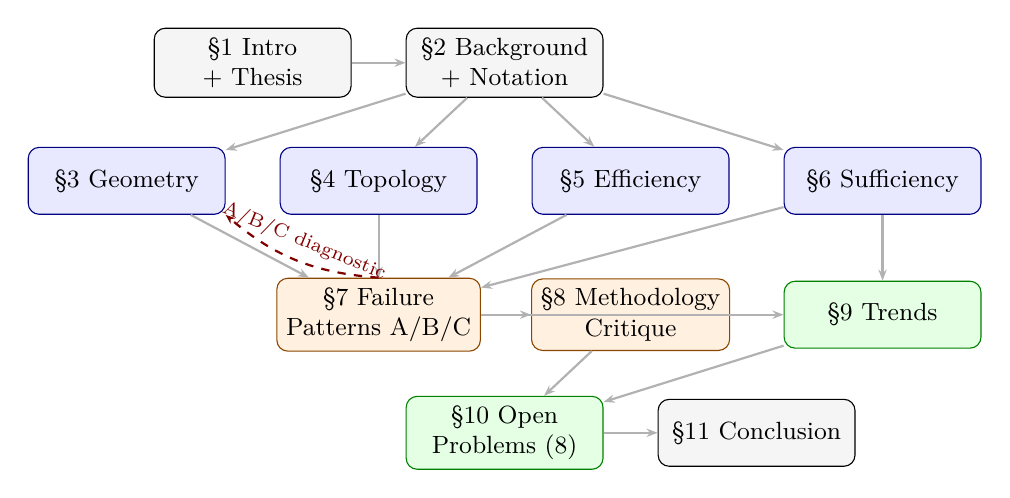
\begin{tikzpicture}[
  sec/.style = {draw, rounded corners=4pt, minimum width=2.5cm,
                minimum height=0.85cm, align=center, font=\small,
                fill=gray!8},
  axis/.style = {sec, fill=blue!9, draw=blue!50!black},
  diag/.style = {sec, fill=orange!12, draw=orange!55!black},
  synth/.style = {sec, fill=green!10, draw=green!50!black},
  arr/.style = {-{Stealth[length=4pt]}, thick, gray!60},
  feed/.style = {-{Stealth[length=3.5pt]}, thick, dashed, red!50!black},
]

%% Row 1: Introduction + Background
\node[sec] (s1) at (0, 0) {\S1 Intro\\+ Thesis};
\node[sec] (s2) at (3.2, 0) {\S2 Background\\+ Notation};

%% Row 2: Four Axes
\node[axis] (s3) at (-1.6, -1.5) {\S3 Geometry};
\node[axis] (s4) at (1.6, -1.5) {\S4 Topology};
\node[axis] (s5) at (4.8, -1.5) {\S5 Efficiency};
\node[axis] (s6) at (8.0, -1.5) {\S6 Sufficiency};

%% Row 3: Diagnostic + Trends
\node[diag] (s7) at (1.6, -3.2) {\S7 Failure\\Patterns A/B/C};
\node[diag] (s8) at (4.8, -3.2) {\S8 Methodology\\Critique};
\node[synth] (s9) at (8.0, -3.2) {\S9 Trends};

%% Row 4: Open Problems + Conclusion
\node[synth] (s10) at (3.2, -4.7) {\S10 Open\\Problems (8)};
\node[sec]  (s11) at (6.4, -4.7) {\S11 Conclusion};

%% Forward arrows
\draw[arr] (s1) -- (s2);
\draw[arr] (s2) -- (s3); \draw[arr] (s2) -- (s4);
\draw[arr] (s2) -- (s5); \draw[arr] (s2) -- (s6);
\draw[arr] (s3) -- (s7); \draw[arr] (s4) -- (s7);
\draw[arr] (s5) -- (s7); \draw[arr] (s6) -- (s7);
\draw[arr] (s7) -- (s8);
\draw[arr] (s6) -- (s9);
\draw[arr] (s7) -- (s9);
\draw[arr] (s8) -- (s10);
\draw[arr] (s9) -- (s10);
\draw[arr] (s10) -- (s11);

%% Feedback arrows (failure patterns feed back to axes)
\draw[feed] (s7.north) to[bend left=18] node[font=\scriptsize, above, sloped]
  {A/B/C diagnostic} (s3.south east);

\end{tikzpicture}
\caption{Bird's-eye view of the survey structure.  Blue boxes: the four
survey axes (Sections~\ref{sec:geometry}--\ref{sec:sufficiency}).  Orange
boxes: the diagnostic programme (failure patterns and methodology critique).
Green boxes: synthesis (trends and open problems).  Dashed arrow: the A/B/C
failure-pattern diagnostic feeds back into the assessment of each axis.}
\label{fig:roadmap}
\end{figure*}

\begin{figure*}[pos=!htbp]
\centering
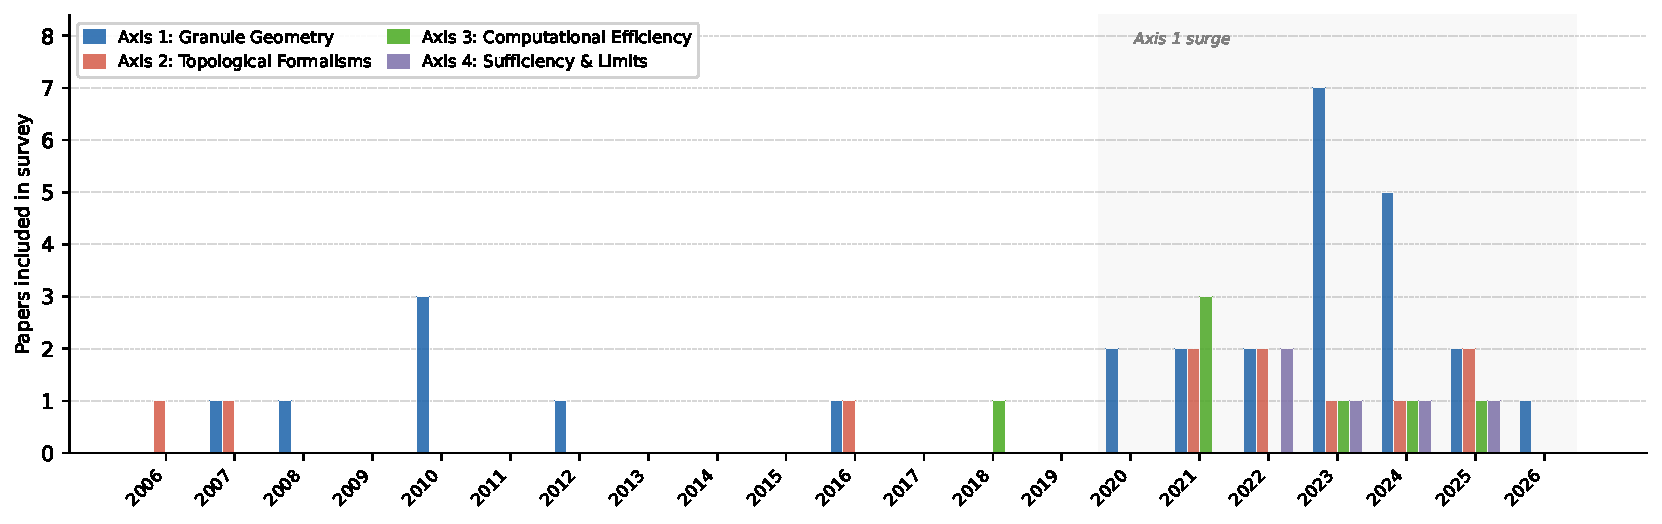
\includegraphics[width=\textwidth]{figures/activity_by_axis.pdf}
\caption{Publication-year distribution of the 52 included papers across the
four research axes (2006--2026).  Background and foundational references
(11 papers: TDA stability theorems, learning-theory bounds, survey references)
are not plotted.  Axis~1 (Granule Geometry) dominates output since 2020,
supporting the saturation argument of Section~\ref{sec:saturation}.
The shaded region marks the 2020--2026 surge period.}
\label{fig:activity}
\end{figure*}

\section{Background and Unified Notation}
\label{sec:background}

We fix notation used throughout the survey.  Readers familiar with
neighbourhood rough sets may skim this section and refer back as needed.
For an introduction to rough sets and their algebraic properties,
see Pawlak and Skowron~\cite{PawlakSkowron2007rudiments}.  Yao~\cite{Yao1998NRS}
establishes the relational semantics for neighbourhood operators: an
$\varepsilon$-ball neighbourhood system is a binary-relation-based approximation
space, and the equivalence or tolerance type of the relation governs which
algebraic properties (reflexivity, symmetry, transitivity) the approximation
operators satisfy.

\paragraph{Symbol overloading: $\delta$.}
The symbol $\delta$ appears in three distinct roles across the survey
(in four notational forms); Table~\ref{tab:delta_uses} lists each.
The NRS radius $\delta$ (Definition~\ref{def:nb}) is a data-structure
parameter chosen by the user and occasionally written explicitly as a
superscript in $\NB{B}^\delta(x)$; Al-shami's $\delta$-open sets
(Section~\ref{sec:abstract_topo}) are a topological concept unrelated to
the metric radius; the confidence $\delta$ in conformal and PAC bounds
(Section~\ref{sec:sufficiency}) is a probability bound.
Similarly, $d$ denotes the decision attribute ($d\colon\U\to\mathcal{D}$)
but also appears as the number of condition attributes (i.e., $|\C| = m$,
though we sometimes write $d$ in its common machine-learning sense of
``dimensionality''); context and notation ($d$ vs.\ $m$) disambiguate.

\begin{table}[pos=!htbp]
\caption{Four distinct uses of $\delta$ in this survey.}
\label{tab:delta_uses}
\centering\small
\begin{tabular}{lll}
\toprule
Context & Meaning & Scope \\
\midrule
Definition~\ref{def:nb} (NRS) & neighbourhood radius $\rho(B(x),B(y))\leq\delta$ & §\ref{sec:background}–§\ref{sec:failure} \\
$\NB{B}^\delta(x)$ shorthand  & same radius as above, made explicit & §\ref{sec:background} only \\
Al-shami $\delta$-open sets   & topological separation axiom parameter & §\ref{sec:abstract_topo} \\
PAC confidence $\delta$        & failure probability bound ($P[\cdot]\leq\delta$) & §\ref{sec:sufficiency} \\
\bottomrule
\end{tabular}
\end{table}

%-----------------------------------------------------------------------
\subsection{Decision Table and Granulation}
\label{sec:notation}
%-----------------------------------------------------------------------

A \emph{decision table} is a tuple $\mathcal{S} = (\U, \C \cup \{d\})$ where
$\U = \{x_1,\ldots,x_n\}$ is a finite universe of objects,
$\C = \{a_1,\ldots,a_m\}$ is a set of condition attributes,
and $d\colon\U \to \mathcal{D}$ is a decision attribute with $|\mathcal{D}|$
classes.  We write $a(x)$ for the value of attribute $a$ on object $x$.

\begin{definition}[Neighbourhood granule]
\label{def:nb}
Given a subset $B \subseteq \C$ and a metric $\rho$ on $\mathbb{R}^{|B|}$,
the \emph{neighbourhood granule} of $x$ at radius $\delta>0$ is
\begin{equation}\label{eq:nb}
  \NB{B}(x) = \{y \in \U : \rho(B(x), B(y)) \leq \delta\},
\end{equation}
where $B(x)$ denotes the projection of $x$ onto the coordinates in $B$.
The pair $(\U, \NB{B})$ is a \emph{neighbourhood approximation space}.
\end{definition}

\begin{definition}[Approximations and positive region]
\label{def:dep}
The \emph{lower} and \emph{upper approximations} of decision class
$Y_k = d^{-1}(k)$ under $B$ are
\begin{equation}\label{eq:approx}
  \LOW_B(Y_k) = \{x \in \U : \NB{B}(x) \subseteq Y_k\}, \quad
  \UPP_B(Y_k) = \{x \in \U : \NB{B}(x) \cap Y_k \neq \emptyset\}.
\end{equation}
The \emph{positive region} and \emph{dependency degree} are
\begin{equation}\label{eq:dep}
  \POS_B(d) = \bigcup_{k} \LOW_B(Y_k), \quad
  \DEP(B) = \frac{|\POS_B(d)|}{|\U|} \in [0,1].
\end{equation}
\end{definition}

The dependency degree $\DEP(B)$ measures the proportion of objects whose
class membership is determined without ambiguity by neighbourhood granules
under $B$.

\begin{definition}[Reduct]
A subset $R \subseteq \C$ is a \emph{reduct} if (i) $\DEP(R) = \DEP(\C)$
and (ii) no proper subset of $R$ satisfies (i).
\end{definition}

The reduct problem is NP-hard in general~\cite{Skowron1992}; practical
algorithms use forward greedy search or heuristics based on attribute
significance $\mathrm{Sig}(a, B, d) = \DEP(B \cup \{a\}) - \DEP(B)$.

%-----------------------------------------------------------------------
\subsection{Granular Ball Extension}
\label{sec:gbnrs}
%-----------------------------------------------------------------------

\emph{Granular ball neighbourhood rough sets} (GBNRS)~\cite{Xia2020GBNRS}
replace the fixed-radius neighbourhood by an adaptive ball fitted per object.
A granular ball $\mathrm{GB}_i$ covering object $x_i$ is characterised by
its centre $c_i$, radius $r_i$, and purity
$p_i = \max_k |Y_k \cap \mathrm{GB}_i| / |\mathrm{GB}_i|$.
Balls with $p_i \geq \tau$ (default $\tau = 2/3$) define the neighbourhood
$\NB{B}^{\mathrm{GB}}(x_i) = \mathrm{GB}_i$.  This yields smaller boundary
regions and faster attribute reduction than fixed-$\delta$ NRS.

%-----------------------------------------------------------------------
\subsection{Evaluation Protocol}
\label{sec:protocol}
%-----------------------------------------------------------------------

To ensure comparability across the experiments in Section~\ref{sec:failure},
we follow a fixed evaluation harness:
\begin{itemize}
  \item Classifiers: 3-NN (Euclidean, $k=3$) and SVM-RBF
        (RBF kernel, $C=1$, $\gamma=\text{scale}$), no hyperparameter tuning.
  \item Validation: stratified 5-fold cross-validation, five independent
        random seeds; results recorded per fold.
  \item Feature-importance metrics are reported in two distinct settings,
        which we keep separate throughout.  (i)~For the \emph{ranking}
        comparisons of Section~\ref{sec:patB}, each of the five seeds draws
        a single 80\% subsample of the dataset without replacement
        (not a bootstrap), giving five importance vectors per method and
        dataset; this is what \texttt{raw\_importance.csv} records, one row
        per (dataset, method, attribute, seed).  (ii)~For every
        \emph{downstream accuracy}, the importance ranking is recomputed
        from scratch on the training partition of each cross-validation
        fold and applied to the held-out partition, so no test object
        influences the selection that is later evaluated on it; this is
        what \texttt{raw\_downstream.csv} records, one row per
        (dataset, method, $k$, seed, fold).  NRS importance
        is implemented as $k$-NN label consistency ($k=7$); this
        is the standard finite-sample surrogate for the $\delta$-ball
        definition when the optimal $\delta$ is unknown.  Setting $k=7$
        corresponds to an implicit, sample-dependent $\delta$ equal to
        the distance to the 7th nearest neighbour; varying $k$ would change
        the effective resolution of the granule and, potentially, the
        importance ranking.  We use a single $k$ throughout, consistent
        with the literature's practice, and note this as a limitation
        (Section~\ref{sec:limitations}).
  \item Datasets: ten UCI benchmarks (Iris, Wine, Ionosphere, Sonar,
        Glass, Ecoli, Heart, Parkinsons, Seeds, WDBC),
        z-score standardised, capped at $n \leq 600$.
  \item Timing: \texttt{time\_reduct\_sec} and \texttt{time\_eval\_sec}
        recorded separately; reported as medians across folds.
\end{itemize}

All raw results (\texttt{raw\_importance.csv}, \texttt{raw\_downstream.csv},
\texttt{raw\_structure.csv}, and \texttt{raw\_knn\_scale.csv} for the
metric-scale ablation of Section~\ref{sec:patC}) are released with this
paper.  Every number in
Sections~\ref{sec:failure}--\ref{sec:methodology} is derived from these CSVs
by the released script \texttt{gen\_tables.py}, and the companion script
\texttt{verify\_tables.py} re-reads the typeset \texttt{.tex} sources and
checks each printed value against a fresh recomputation from the raw data,
so that a drift between the manuscript and the released data fails
audibly rather than silently.  Standard deviations are always computed from
the per-fold values, never reconstructed from rounded summaries.  One
convention is worth flagging for anyone reproducing the bound of
Theorem~\ref{thm:pai_bound}: the column \texttt{pai\_bound} stores
$(d_{\max}+1)\,\mathrm{range}(a_j)$, the bound for the summed score, not the
sharper per-dimension quantity $\mathrm{range}(a_j)$.

%-----------------------------------------------------------------------
\subsection{Persistent Homology (Brief Review)}
\label{sec:ph}
%-----------------------------------------------------------------------

We summarise persistent homology to the degree needed for
Sections~\ref{sec:topology} and~\ref{sec:failure}; readers seeking a full
treatment are referred to~\cite{Edelsbrunner2010} or the survey~\cite{Su2025TDA}.

Given a point cloud $X \subset \mathbb{R}^d$, the Vietoris--Rips filtration
$\{VR_\varepsilon\}_{\varepsilon \geq 0}$ is a nested sequence of simplicial
complexes: $\sigma \in VR_\varepsilon$ iff all pairwise distances between
its vertices are $\leq \varepsilon$.  As $\varepsilon$ increases, topological
features (connected components, loops, voids) are born and later die.
The \emph{persistence diagram} $\mathrm{Dgm}_k(X)$ is the multiset of
$(b,d)$ pairs recording birth and death of $k$-dimensional features.
$\mathrm{Dgm}_0$ tracks connected components; $\mathrm{Dgm}_1$ tracks loops.

The \emph{bottleneck distance} $d_B(\mathrm{Dgm}(X), \mathrm{Dgm}(Y))$ is
the infimum over matchings between the two diagrams of the maximum unmatched
point offset.  Chazal et al.'s stability theorem guarantees
$d_B(\mathrm{Dgm}(X), \mathrm{Dgm}(Y)) \leq 2\,d_H(X,Y)$
for Vietoris--Rips filtrations, where $d_H$ is the Hausdorff
distance~\cite{Chazal2009Stability,CohenSteiner2007stability}.
(For \v{C}ech filtrations the factor 2 is absent; we use Rips throughout.)
This stability guarantee plays a central role in Pattern~B
(Section~\ref{sec:patB}).

\section{Axis 1: Granule Geometry}
\label{sec:geometry}

The oldest and most active research axis in modern GrC concerns the
\emph{shape} of the granule $\NB{B}(x)$.  Pawlak's original rough sets use
equivalence classes---granules shaped by a partition, with no notion of
proximity~\cite{Pawlak1982}.  The introduction of neighbourhood rough sets
(NRS) by Hu et al.~\cite{Hu2008NRS} replaced the partition with a fixed-radius
ball in feature space, enabling continuous and mixed-type attributes.
Yao's triarchic theory~\cite{Yao2016triarchic} situates this axis within a
three-tier taxonomy of GrC: information granules (the balls themselves),
granular structures (the neighbourhood system induced by a ball geometry),
and granular computing methods (attribute reduction algorithms operating on that
structure) are treated as interdependent design choices.
The first major deformation replaced the crisp $\delta$-cut with a graded
membership function: \emph{fuzzy-rough NRS}~\cite{JensenShen2007TFS,Cornelis2010IS}
lets objects partially belong to a neighbourhood, so the lower approximation
becomes a fuzzy set and attribute importance is computed via graded positive
regions.  This bridge between classical NRS and the adaptive granular balls
described below remains the most-cited line within the geometry axis.
The subsequent decade has been a systematic exploration of every natural
deformation of that ball.

%-----------------------------------------------------------------------
\subsection{Taxonomy of Granule Geometries}
\label{sec:geo_taxonomy}
%-----------------------------------------------------------------------

Table~\ref{tab:granule_tax} organises the literature by what geometric
constraint is relaxed and what is gained.  We restrict this table to
\emph{metric-space} neighbourhood granules; dominance-based rough sets
(Greco, Matarazzo, and S\l{}owi\'nski, 2001; $>$1\,600 citations) use
ordinal preference structures rather than metric balls and are outside
this scope.  Reading across columns,
three patterns emerge.  First, each major deformation originates from a
single highly-cited paper that accumulates most follow-on citations
(Hu~\cite{Hu2008NRS}, Xia~\cite{Xia2020GBNRS}) while the surrounding
variants remain modestly cited.  Second, the ``Benefit claimed'' column
is nearly invariant: every row asserts a smaller boundary region,
faster computation, or both---the field's two standard metrics.  Third,
the ``Key mechanism'' column exhausts the natural degrees of freedom
(ball shape, radius adaptation, purity threshold, aggregation rule, and
weighting scheme); the final entries combine multiple mechanisms rather
than introducing new ones, which is a typical signal of axis saturation.

\begin{table*}[pos=!htbp]
\caption{Taxonomy of granule geometries in neighbourhood rough sets
(2007--2026).  ``Adaptive'' means the granule radius or shape varies
per object.  All citations refer to the literature log.}
\label{tab:granule_tax}
\centering\small
\setlength\tabcolsep{4pt}
\begin{tabular}{p{4.0cm}p{5.6cm}p{4.2cm}p{1.4cm}r}
\toprule
Granule type & Key mechanism & Benefit claimed & Venue & Cites \\
\midrule
Fixed-radius ball (NRS)~\cite{Hu2008NRS}
  & Euclidean $\delta$-ball
  & Handles continuous data
  & TKDE'08 & --- \\
\addlinespace
Fuzzy-rough NRS~\cite{JensenShen2007TFS,Cornelis2010IS}
  & Graded membership replaces crisp $\delta$-cut; fuzzy lower approximation
  & Handles overlapping boundary; graded attribute importance
  & TFS'07 & 467 \\
\addlinespace
Adaptive ball (GBNRS)~\cite{Xia2020GBNRS}
  & Purity $\geq\tau$ controls radius per object
  & Smaller boundary region; faster
  & TKDE'20 & 259 \\
\addlinespace
Efficient GB generation~\cite{Xia2022EfficientGB}
  & Optimised splitting for tighter balls
  & Faster, more accurate than GBNRS
  & TNNLS'22 & 143 \\
\addlinespace
Unified GB (GBRS)~\cite{Xia2023GBRS}
  & GB subsumes both Pawlak RS and NRS
  & Common framework; single algorithm
  & TNNLS'23 & 77 \\
\addlinespace
Three-way + GB~\cite{Xia2024TFS3WC}
  & Uncertainty-based three-way decision on GB
  & Deferred classification; lower error
  & TFS'24 & 87 \\
\addlinespace
Directional semi-ball~\cite{Qian2024directional}
  & Half-ball oriented toward same-class samples
  & Better near class boundary
  & IJMLC'24 & 16 \\
\addlinespace
Bi-directional adaptive ball~\cite{Ju2023bidirectional}
  & Forward+backward $k$-NN; justifiable granularity
  & Adaptive $k$ per object; Dempster-Shafer
  & IJAR'23 & 12 \\
\addlinespace
Multi-granularity neighbour (MGNR)~\cite{Xie2024TPAMI}
  & Multiple granularity levels simultaneously
  & Richer neighbourhood representation; superior on large-scale benchmarks
  & TPAMI'24 & 57 \\
\addlinespace
Fuzzy granular ball~\cite{Sun2024TFS}
  & Fuzzy neighbourhood inside GB
  & Sparse/noisy samples handled
  & TFS'24 & 26 \\
\addlinespace
Multi-scale GB + ANN~\cite{Zhang2025NN}
  & Different scales for different attributes; ANN weights
  & Weight variation across scales
  & NeurNet'25 & 7 \\
\addlinespace
Adaptive fuzzy multineighbourhood GB~\cite{Sun2025EAAI}
  & Per-feature max/min std for radius set; label enhancement
  & Multi-label + label enhancement
  & EAAI'25 & 15 \\
\addlinespace
GB + three-way approximations (MGFE)~\cite{XiaDeyou2024TFS}
  & GB compresses sample space; fuzzy entropy on representative
  & Efficient filter-wrapper
  & TFS'24 & 21 \\
\addlinespace
VPGB (variable-precision GB)~\cite{Peng2022VPGB}
  & Purity threshold relaxed for noise
  & Robust to label noise
  & InfSci'22 & 46 \\
\addlinespace
GB guided selector~\cite{Xia2021KBSselector}
  & GB as initialiser for greedy search
  & Fewer significance evaluations
  & KBS'21 & 49 \\
\addlinespace
Weighted $k$-NN NRS~\cite{Wang2023ESWA}
  & Per-sample weight from std of neighbour labels
  & Noise-sensitive boundary region reduced
  & ESWA'23 & 66 \\
\addlinespace
Neighbourhood self-information~\cite{Wang2020selfinfo}
  & Combines lower and upper approximation uncertainty
  & Better feature scoring than dependency alone
  & Trans.Cyber.'20 & 227 \\
\addlinespace
Weighted NRS~\cite{Hu2021WNRS}
  & Pre-computed attribute--decision correlation sets weights in $\rho$
  & Weights guide radius; isometric search for optimal $\delta$
  & KBS'21 & 138 \\
\addlinespace
Param-free homogeneous granules (MHMG)~\cite{Nguyen2026MHMG}
  & Log-sum knowledge energy + maximal class-pure granule; no $\delta$
  & Eliminates radius tuning; 93.2\% reduction on 12 UCI sets
  & IJAR'26 & --- \\
\addlinespace
Multigranulation NRS~\cite{QianLiangYaoDang2010MGRS,LinQianLi2012NMGRS}
  & Multiple binary relations each generate a neighbourhood; union/intersection
  & Handles heterogeneous granularity sources
  & InfSci'10 & 742 \\
\addlinespace
Justified granularity~\cite{Li2023TFS}
  & Fuzzy C-means + justified-granularity principle selects optimal ball size
  & Principled radius from data density; no manual threshold
  & TFS'23 & 121 \\
\bottomrule
\end{tabular}
\end{table*}

%-----------------------------------------------------------------------
\subsection{The Saturation Argument}
\label{sec:saturation}
%-----------------------------------------------------------------------

Of GBNRS's~\cite{Xia2020GBNRS} 259 citing papers, 255 appeared between 2021
and 2026.  Of the top-20 by citation count, 14 appear in
Table~\ref{tab:granule_tax}; the remainder are clustering and anomaly-detection
applications outside feature selection.  The six deformation axes in Table~\ref{tab:granule_tax} (shape, scale,
purity, aggregation, weighting, neighbourhood type) have each been explored
by multiple groups; finding a seventh axis that produces a non-trivial
contribution appears increasingly difficult.

\begin{itemize}
  \item \emph{Shape}: Euclidean (crisp) ball $\to$ fuzzy-membership ball
        (Jensen \& Shen~\cite{JensenShen2007TFS}) $\to$ half-ball (directional,
        Qian et al.~\cite{Qian2024directional}) $\to$ bidirectional ball
        (Ju et al.~\cite{Ju2023bidirectional}) $\to$ fuzzy granular ball (Sun et
        al.~\cite{Sun2024TFS}).
  \item \emph{Scale}: fixed radius $\to$ per-object purity-controlled
        (GBNRS~\cite{Xia2020GBNRS}) $\to$ multi-scale (Zhang et
        al.~\cite{Zhang2025NN}) $\to$ three-way approximation scale
        (Xia et al.~\cite{XiaDeyou2024TFS}).
  \item \emph{Label regime}: single label $\to$ noisy label
        (VPGB~\cite{Peng2022VPGB}) $\to$ partial label
        (Qian et al.~\cite{Qian2023InfoFusion}) $\to$ label distribution
        (Qian et al.~\cite{Sun2023KBS}) $\to$ dynamic/incremental update
        (Zhang et al.~\cite{Zhang2023TKDEincremental}).
  \item \emph{Framework extension}: standalone $\to$ unified with Pawlak RS
        (GBRS~\cite{Xia2023GBRS}) $\to$ three-way decision
        (3WC-GBNRS++~\cite{Xia2024TFS3WC}).  The three-way decision framework
        itself was formalised by Yao~\cite{Yao2010threeway} as a cost-minimising
        Bayesian decision that partitions objects into positive, negative, and
        boundary regions under a probabilistic rough set model.
\end{itemize}

Figure~\ref{fig:saturation} maps the four deformation axes as a roadmap;
the four bullet points below annotate each axis.

\begin{figure*}[pos=!htbp]
\centering
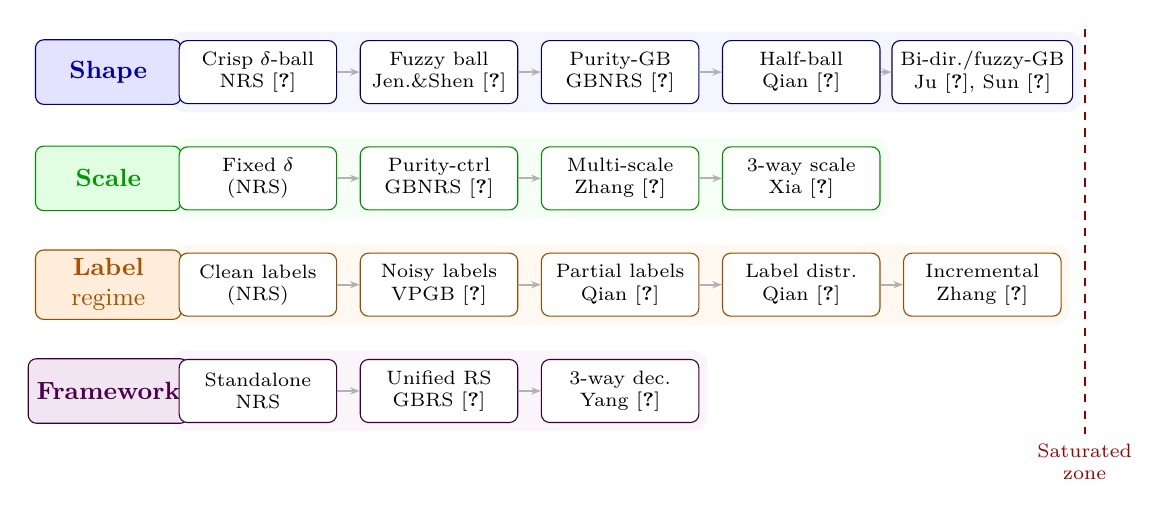
\begin{tikzpicture}[
  lbl/.style   = {draw, rounded corners=3pt, minimum width=1.85cm,
                  minimum height=0.82cm, align=center,
                  font=\small, inner sep=3pt},
  shp/.style   = {lbl, fill=blue!11,   draw=blue!50!black,   text=blue!65!black},
  scl/.style   = {lbl, fill=green!11,  draw=green!55!black,  text=green!60!black},
  lab/.style   = {lbl, fill=orange!14, draw=orange!60!black, text=orange!65!black},
  frm/.style   = {lbl, fill=violet!10, draw=violet!45!black, text=violet!60!black},
  mile/.style  = {draw, rounded corners=3pt, fill=white, draw=gray!50,
                  minimum width=2.00cm, minimum height=0.80cm, align=center,
                  font=\scriptsize, inner sep=3pt},
  mshp/.style  = {mile, draw=blue!45!black},
  mscl/.style  = {mile, draw=green!55!black},
  mlab/.style  = {mile, draw=orange!60!black},
  mfrm/.style  = {mile, draw=violet!45!black},
  arr/.style   = {-{Stealth[length=3.5pt]}, thick, color=gray!60},
  satline/.style = {dashed, red!55!black, thick},
]

%% ── Lane labels ─────────────────────────────────────────────────────────────
\node[shp] at (-1.05, 3.05) {\textbf{Shape}};
\node[scl] at (-1.05, 1.70) {\textbf{Scale}};
\node[lab] at (-1.05, 0.35) {\textbf{Label}\\regime};
\node[frm] at (-1.05,-1.00) {\textbf{Framework}};

%% ── Shape lane  (y = 3.05) ──────────────────────────────────────────────────
\node[mshp] (SA1) at ( 0.85, 3.05) {Crisp $\delta$-ball\\NRS~\cite{Hu2008NRS}};
\node[mshp] (SA2) at ( 3.15, 3.05) {Fuzzy ball\\Jen.\&Shen~\cite{JensenShen2007TFS}};
\node[mshp] (SA3) at ( 5.45, 3.05) {Purity-GB\\GBNRS~\cite{Xia2020GBNRS}};
\node[mshp] (SA4) at ( 7.75, 3.05) {Half-ball\\Qian~\cite{Qian2024directional}};
\node[mshp] (SA5) at (10.05, 3.05) {Bi-dir./fuzzy-GB\\Ju~\cite{Ju2023bidirectional}, Sun~\cite{Sun2024TFS}};
\draw[arr] (SA1)--(SA2); \draw[arr] (SA2)--(SA3);
\draw[arr] (SA3)--(SA4); \draw[arr] (SA4)--(SA5);

%% ── Scale lane  (y = 1.70) ──────────────────────────────────────────────────
\node[mscl] (SB1) at ( 0.85, 1.70) {Fixed $\delta$\\(NRS)};
\node[mscl] (SB2) at ( 3.15, 1.70) {Purity-ctrl\\GBNRS~\cite{Xia2020GBNRS}};
\node[mscl] (SB3) at ( 5.45, 1.70) {Multi-scale\\Zhang~\cite{Zhang2025NN}};
\node[mscl] (SB4) at ( 7.75, 1.70) {3-way scale\\Xia~\cite{XiaDeyou2024TFS}};
\draw[arr] (SB1)--(SB2); \draw[arr] (SB2)--(SB3); \draw[arr] (SB3)--(SB4);

%% ── Label regime lane  (y = 0.35) ───────────────────────────────────────────
\node[mlab] (SC1) at ( 0.85, 0.35) {Clean labels\\(NRS)};
\node[mlab] (SC2) at ( 3.15, 0.35) {Noisy labels\\VPGB~\cite{Peng2022VPGB}};
\node[mlab] (SC3) at ( 5.45, 0.35) {Partial labels\\Qian~\cite{Qian2023InfoFusion}};
\node[mlab] (SC4) at ( 7.75, 0.35) {Label distr.\\Qian~\cite{Sun2023KBS}};
\node[mlab] (SC5) at (10.05, 0.35) {Incremental\\Zhang~\cite{Zhang2023TKDEincremental}};
\draw[arr] (SC1)--(SC2); \draw[arr] (SC2)--(SC3);
\draw[arr] (SC3)--(SC4); \draw[arr] (SC4)--(SC5);

%% ── Framework lane  (y = -1.00) ─────────────────────────────────────────────
\node[mfrm] (SD1) at (0.85,-1.00) {Standalone\\NRS};
\node[mfrm] (SD2) at (3.15,-1.00) {Unified RS\\GBRS~\cite{Xia2023GBRS}};
\node[mfrm] (SD3) at (5.45,-1.00) {3-way dec.\\Yang~\cite{Xia2024TFS3WC}};
\draw[arr] (SD1)--(SD2); \draw[arr] (SD2)--(SD3);

%% ── Saturation zone vertical marker ─────────────────────────────────────────
\draw[satline] (11.35, 3.60) -- (11.35,-1.55);
\node[font=\scriptsize, text=red!60!black, align=center]
  at (11.35,-1.90) {Saturated\\zone};

%% ── Background shading per lane ─────────────────────────────────────────────
\begin{scope}[on background layer]
  \node[fill=blue!4,   rounded corners=5pt,
        fit=(SA1)(SA2)(SA3)(SA4)(SA5), inner sep=3pt] {};
  \node[fill=green!4,  rounded corners=5pt,
        fit=(SB1)(SB2)(SB3)(SB4), inner sep=3pt] {};
  \node[fill=orange!5, rounded corners=5pt,
        fit=(SC1)(SC2)(SC3)(SC4)(SC5), inner sep=3pt] {};
  \node[fill=violet!4, rounded corners=5pt,
        fit=(SD1)(SD2)(SD3), inner sep=3pt] {};
\end{scope}

\end{tikzpicture}
\caption{Saturation roadmap of the granule geometry axis.  Four deformation
directions are each independently explored to their natural end-state
(rightmost milestone per lane).  The dashed red line marks the saturation
boundary: a new contribution must target a regime not covered by any existing
node, or supply a theoretical guarantee absent across all nodes
(Section~\ref{sec:geo_gaps}).}
\label{fig:saturation}
\end{figure*}

We conclude that the granule geometry axis is saturated: a new
paper proposing yet another geometric deformation of the neighbourhood ball
must now (a) target a specific application regime not covered by any row in
Table~\ref{tab:granule_tax} or any node in Figure~\ref{fig:saturation}, or
(b) offer a theoretical guarantee (e.g., a finite-sample reduction bound)
that none of the existing variants provides.
Absent either condition, reviewers at TKDE, TPAMI, or TFS will ask what is
new.

%-----------------------------------------------------------------------
\subsection{Theoretical Gaps}
\label{sec:geo_gaps}
%-----------------------------------------------------------------------

Despite saturation in geometry, several theoretical questions remain open
and are listed in Section~\ref{sec:open}:

\begin{enumerate}
  \item \emph{Optimal purity threshold.}  GBNRS uses $\tau = 2/3$ without
        a theoretical justification tied to the Bayes error of the problem.
        The connection between $\tau$ and the Bayes error lower bound
        (Section~\ref{sec:sufficiency}) has not been formalised.
  \item \emph{Reduct stability under ball perturbation.}  When $\tau$
        changes slightly, how much can the reduct change?  We found no
        perturbation bound for purity-controlled granular balls in the
        surveyed literature, and none is implied by the fixed-radius
        analyses, whose radius is a parameter rather than a data-dependent
        quantity.
  \item \emph{Concentration of measure.}  At high dimension $d \gg 1$,
        the purity of a ball of fixed expected radius approaches $1/|\mathcal{D}|$
        (maximum impurity) due to concentration of measure.  How does GBNRS
        degrade with $d$?  The literature benchmarks on $d \leq 166$ (Musk1);
        behaviour at $d \sim 10^3$ (genomics) is untested.
\end{enumerate}

%-----------------------------------------------------------------------
\subsection{Emerging Extensions: Incremental and Three-Way Decision}
\label{sec:geo_emerging}
%-----------------------------------------------------------------------

Two active extensions of the granule geometry axis differ from the deformations
surveyed above: they do not change the shape of the granule but change
when or \emph{how} the reduct decision is applied.

\paragraph{Incremental feature selection.}
When data arrive in batches or streams, recomputing the full reduct after each
update is prohibitively expensive: a forward-greedy search on $n$ objects and
$d$ attributes requires $O(n^2 d)$ significance evaluations per run.
Incremental algorithms maintain a previously-found reduct $R_t$ and adjust it
locally when a batch $\Delta\mathcal{U}$ arrives or departs, updating only the
granular balls whose purity is altered by the new objects.
Zhang et al.~\cite{Zhang2023TKDEincremental} apply this strategy to GB-NRS,
achieving near-constant update cost when $|\Delta\mathcal{U}| \ll n$.
The practical gain is substantial; however, a critical question is unanswered:
does the locally-updated reduct $R_{t+1}$ coincide with the reduct that a full
re-run on $\mathcal{U} \cup \Delta\mathcal{U}$ would have found?
No existing paper bounds the deviation $|R_{t+1} \setminus R^*| + |R^* \setminus R_{t+1}|$,
where $R^*$ is the globally optimal reduct.
Incremental papers typically report only wall-clock speedup, not reduct quality
loss---a Pattern~C risk: the method wins on the metric it directly optimises
(time) but leaves the accuracy-vs-reduct-size trade-off unverified.

\paragraph{Three-way decision integration.}
The three-way decision (3WD) framework, formalised by
Yao~\cite{Yao2010threeway} as a cost-minimising Bayesian partition, replaces
the binary positive/negative split with three regions: positive ($\mathrm{POS}$,
accept), negative ($\mathrm{NEG}$, reject), and boundary ($\mathrm{BND}$,
defer).  Objects in $\mathrm{BND}$ receive no label until additional information
is gathered.  This is not a geometric deformation of the granule; it is a
change in the \emph{payoff function} applied after the granule is built.
Yang et al.~\cite{Xia2024TFS3WC} integrate 3WD with GBNRS by using the
granule's purity to determine region membership under a non-uniform cost matrix.
Two pattern risks arise.
First (Pattern~A): when $\tau = 1$ and costs are symmetric, the 3WD boundary
region collapses to the NRS positive region---the 3WD layer adds nothing.
The contribution is non-trivial only when the cost matrix is genuinely
asymmetric and $\tau$ is calibrated from domain knowledge.
Second (Pattern~C): 3WD methods are typically evaluated on cost-sensitive
accuracy under a self-chosen cost matrix, not on standard 0-1 accuracy.
Excluding boundary objects from accuracy computation inflates results on the
remaining objects.  A fair comparison requires reporting both the boundary
region size and 0-1 accuracy on the full dataset.
Where cost asymmetry is real---medical diagnosis, intrusion detection---3WD-GrC
is a principled and useful approach; the open question is how to derive cost
matrices from data rather than assigning them by hand
(Section~\ref{sec:open}).

\section{Axis 2: Topological Formalisms}
\label{sec:topology}

Topology enters granular computing through two research communities that
develop largely independently.  We call them the \emph{abstract topology}
branch and the \emph{computational topology (TDA)} branch.  Mapping this
split is one of the original contributions of this survey.

We state the separation as a bounded, checkable claim rather than as a
universal one.  Within the corpus assembled by the search protocol of
Appendix~\ref{app:search}, no paper cites work from both branches, and we
found none in either branch's reference list that reaches into the other.
This is a statement about a 52-paper corpus retrieved from OpenAlex and
Google Scholar in September 2025, not a proof that no such paper exists
anywhere: the two branches publish in disjoint venue sets, and a bridging
paper in a venue outside our search frame would not have been retrieved.
What the corpus does establish is that the bridge is rare enough to be
absent from the literature a researcher entering this area would find.

%-----------------------------------------------------------------------
\subsection{Branch A: Abstract Topology}
\label{sec:abstract_topo}
%-----------------------------------------------------------------------

Abstract topology treats the neighbourhood operator $\NB{B}$ as a
topological structure and asks: which axioms does it satisfy?  What is the
algebraic relationship between the lower/upper approximation operators and
classical topological operators (interior, closure)?  When do two different
neighbourhood systems produce the same approximation operators?

\paragraph{Foundational work.}
Zhu~\cite{Zhu2007covering} established covering rough sets from the topological
viewpoint: a \emph{covering} of $\U$ generates a neighbourhood system; the
paper characterises when two coverings share the same lower (or upper)
approximation operator, and constructs complete axiomatic systems for both.
With 637 citations, this is the most-cited Axis~2 paper in this survey.
D'eer et al.~\cite{DeerCornelisYao2016} later showed that several
covering-based rough set models in the literature are semantically unsound---they
fail to reduce to Pawlak rough sets when the covering is a partition---and
proposed corrected definitions that preserve the algebraic link to the
original framework.

Yao~\cite{Yao2023Alexandrov} identifies the Alexandrov topology as the
unifying structure: a preorder $\preceq$ on $\U$ induces an Alexandrov
topology whose specialisation preorder recovers $\preceq$.  Under this lens,
the four main rough set models (binary-relation, neighbourhood-operator,
covering, subset-system) are all instances of the same topological framework,
distinguished only by which axioms (reflexivity, transitivity, symmetry) the
preorder satisfies.

\paragraph{Separation axioms.}
A parallel line studies which topological separation axioms (T$_0$ through
T$_4$) are satisfied by the approximation space induced by an equivalence or
neighbourhood relation, and whether stronger axioms correspond to better
approximation quality (smaller boundary region).  The common thread across
four recent papers---Al-shami et al.~\cite{AlShami2025delta} ($\delta$-open
sets), Al-shami~\cite{AlShami2022topology} (somewhat-open sets via
$N_\rho$-neighbourhoods), Al-shami and Alshammari~\cite{AlShami2022supra}
(supra-topology), and El~Safty~\cite{ElSafty2021}
(simply$^*\alpha$-open sets)---is the progressive weakening of the open-set
axiom: each relaxation yields coarser granules and therefore a smaller
boundary region, at the cost of weaker algebraic properties.  None of
these papers benchmarks the resulting approximation against NRS/GBNRS at
the scale of Section~\ref{sec:methodology}'s recommended protocol, so
the practical magnitude of the boundary-region improvement remains
unquantified.

\paragraph{Fuzzy topology.}
Lai and Zhang's~\cite{LaiZhang2006} equivalence between fuzzy preorders and
fuzzy Alexandrov topologies provides a bridge to fuzzy rough sets: an $\alpha$-cut
of a fuzzy similarity relation $R$ yields a crisp partition at threshold
$\alpha$, and the resulting nested family of partitions defines a fuzzy
topology on $\U$.  The authors' prior work~\cite{DaiTT2024IFT} exploits
this structure by building an \emph{intuitionistic} fuzzy topology (IFT)
from a pre-order relation, then using the IFT subbasis to measure attribute
significance; the paper reports reducts 50\% smaller on average than
dependency-based NRS, with 10\% higher accuracy.
Applying this survey's own diagnostic: the IFT subbasis significance measure
is a monotone function of the pre-order's $\alpha$-cut chain---placing it in
the Pattern~A risk zone (reduction to NRS dependency at the cut-threshold).
The 50\%/10\% figures are also reported without significance testing, raising
the Pattern~C concern; we flag these as claims requiring independent
verification rather than taking them at face value.

\paragraph{Assessment of the abstract branch.}
The abstract topology branch is mathematically mature.  Its primary
contribution has been taxonomic: clarifying which set-theoretic properties
of an approximation operator correspond to which topological axioms.  The
computational payoff---smaller reducts, better accuracy---is reported in
isolated papers but has not been benchmarked systematically against modern
NRS/GBNRS at the scale and with the rigour advocated in
Section~\ref{sec:methodology}.

%-----------------------------------------------------------------------
\subsection{Branch B: Computational Topology (TDA)}
\label{sec:tda}
%-----------------------------------------------------------------------

The TDA branch uses \emph{persistent homology} (Section~\ref{sec:ph}) as
a computational tool and asks: can the topological summary of a dataset
generate neighbourhoods, identify important attributes, or define a rough
approximation space?

\paragraph{Background.}
Carlsson~\cite{Carlsson2009topology} established persistent homology as a
tool for data analysis, showing that the birth/death intervals of topological
features across scale form a stable, discriminative summary;
Ghrist~\cite{Ghrist2008barcodes} introduced the \emph{barcode} representation
that encodes these intervals compactly.
Chazal and Michel~\cite{ChazalMichel2021TDA} provide a practical introduction
covering filtrations, persistence diagrams, and vectorisation for practitioners;
Otter et al.~\cite{Otter2017roadmap} survey the computational algorithms
for building different filtration types.
Hensel et al.~\cite{HenselMoorRieck2021} survey topological machine learning
methods beyond point-cloud homology, including graph persistence and topological
regularisers in deep learning.  None of these methods interact with rough set
approximation operators.
Pun et al.~\cite{Pun2022PH} survey persistent-homology-based machine learning
across classification, regression, and feature-extraction tasks, and provide
the only systematic comparison of simplicial complex types (alpha vs.\
Vietoris--Rips) and vectorisation strategies.  None of the 50+ methods they
survey are applied to rough-set reducts; this is one of the two cross-branch
gaps this survey maps.

\paragraph{Classifier via simplicial granules.}
Kindelan et al.~\cite{Kindelan2021TDABC} build a filtered simplicial complex
on the dataset, use persistent homology to select a sub-complex that captures
the data's topology, and define each unlabelled point's neighbourhood via its
\emph{star} and \emph{link} operators in the sub-complex.  Labels propagate
from labelled to unlabelled points through these simplicial neighbourhoods.
On eight datasets including imbalanced and overlapping classes, the method
outperforms $k$-NN and weighted $k$-NN.

This is, in the language of granular computing, a method for defining an
\emph{adaptive granule} $\NB{}(x) = \mathrm{star}(x) \cup \mathrm{link}(x)$
from the dataset's topology.  Kindelan et al.\ do not use the language of
rough sets and do not compute reducts or boundary regions; their goal is
classification, not feature selection.

\paragraph{Attribute importance from persistence.}
Our own work (Sections~\ref{sec:patB}--\ref{sec:patC}) tests whether
persistence diagrams can score attribute importance.  Writing
$\mathrm{Dgm}_k(\U_B)$ for the dimension-$k$ persistence diagram of the
Vietoris--Rips filtration built on the projection of $\U$ onto attribute
set $B$, we define the \emph{persistence attribute importance} of $a_j$ as
the total bottleneck displacement caused by deleting that coordinate,
summed over the homological dimensions actually computed:
\begin{equation}\label{eq:pai_def}
  \mathrm{PAI}(j) \;=\; \sum_{k=0}^{d_{\max}}
    d_B\!\left(\mathrm{Dgm}_k(\U_{\C}),\,
               \mathrm{Dgm}_k(\U_{\C\setminus\{j\}})\right),
\end{equation}
with $d_{\max}=1$ throughout (so $H_0$ and $H_1$ contribute).  The sum,
rather than a single diagram distance, is what our implementation computes,
and it is what the following bound is stated for.

\begin{theorem}[PAI upper bound]
\label{thm:pai_bound}
Let $\U$ be a finite point cloud, let all attributes be real-valued, and let
the Vietoris--Rips filtrations be built from the Euclidean metric on the
retained coordinates.  Then
\begin{equation}\label{eq:pai_bound}
  \mathrm{PAI}(j) \leq (d_{\max}+1)\,\mathrm{range}(a_j),
\end{equation}
where $\mathrm{range}(a_j) = \max_{x\in\U} a_j(x) - \min_{x\in\U} a_j(x)$.
Moreover each individual summand in~\eqref{eq:pai_def} obeys the sharper
bound $d_B(\mathrm{Dgm}_k(\U_{\C}),\mathrm{Dgm}_k(\U_{\C\setminus\{j\}}))
\leq \mathrm{range}(a_j)$.
\end{theorem}

\begin{proof}
Let $d_{\C}$ and $d_{\C\setminus\{j\}}$ denote the pairwise Euclidean distance
functions on $\U$ induced by attribute sets $\C$ and $\C\setminus\{j\}$.  For
any $x,y\in\U$, writing $S=\sum_{a_i\in\C\setminus\{j\}}(a_i(x)-a_i(y))^2$ and
$t=(a_j(x)-a_j(y))^2$, subadditivity of the square root gives
$\sqrt{S+t}-\sqrt{S}\leq\sqrt{t}$, so
\[
  0 \;\leq\; d_{\C}(x,y) - d_{\C\setminus\{j\}}(x,y)
    \;\leq\; |a_j(x)-a_j(y)| \;\leq\; \mathrm{range}(a_j),
\]
hence $\|d_{\C}-d_{\C\setminus\{j\}}\|_\infty \leq \mathrm{range}(a_j)$.
Two Vietoris--Rips filtrations whose defining distance functions differ by at
most $\varepsilon$ in the supremum norm are $\varepsilon$-interleaved, so by
the algebraic stability theorem for persistence
modules~\cite{CohenSteiner2007stability,Chazal2009Stability} each dimension
satisfies
$d_B(\mathrm{Dgm}_k(\U_{\C}),\mathrm{Dgm}_k(\U_{\C\setminus\{j\}}))
\leq \|d_{\C}-d_{\C\setminus\{j\}}\|_\infty \leq \mathrm{range}(a_j)$.
This is the sharper claim.  Summing it over the $d_{\max}+1$ dimensions
in~\eqref{eq:pai_def} yields~\eqref{eq:pai_bound}.
\end{proof}

The multiplier $(d_{\max}+1)$ is therefore not a property of the Rips
skeleton but simply a count of the terms being summed; a single-dimension
importance score would carry no multiplier.  The released column
\texttt{pai\_bound} in \texttt{raw\_importance.csv} records the right-hand
side of~\eqref{eq:pai_bound}, i.e.\ $2\,\mathrm{range}(a_j)$ at
$d_{\max}=1$.

\begin{remark}[Domain of validity]
\label{rem:pai_domain}
Equation~\eqref{eq:pai_def} presupposes $|\C|\geq 2$: at $d=1$ the reduced
cloud $\U_{\C\setminus\{j\}}$ is empty and PAI is undefined.  The scores are
also invariant to translation of $a_j$ but not to rescaling, which is the
formal source of the measurement-scale special case of Pattern~B
(Section~\ref{sec:patB}).
\end{remark}

The bound is valid but loose: across all ten datasets and five seeds there
are zero violations, with mean ratio
$\mathrm{PAI}(j)/[(d_{\max}+1)\mathrm{range}(a_j)] = 0.038$ (max $0.194$);
against the sharper per-dimension bound the mean ratio is $0.075$
(max $0.387$).  Because it is loose by more than an order of magnitude, the
bound does not by itself imply that PAI tracks range---it is consistent with
that hypothesis and explains why the hypothesis is worth testing.  What the
bound does establish is structural: PAI's admissible magnitude is
proportional to the feature's range, so a feature can score highly for
reasons unrelated to class structure.  Whether range is in fact the dominant
driver is an empirical question, tested directly in Section~\ref{sec:patB}.

\paragraph{Alternative vectorisation strategies.}
The TDA literature offers several vectorisation approaches beyond the
bottleneck distance used in this survey's experiments.  Persistence
landscapes~\cite{Bubenik2015landscapes} map each diagram to a sequence of
piecewise-linear functions amenable to Banach-space statistics; persistence
images~\cite{Adams2017persistence} discretise the birth-death plane into a
stable, fixed-dimensional vector; and the Mapper
algorithm~\cite{Singh2007mapper} produces a simplicial summary of the data's
shape without computing homology.  Pun et al.~\cite{Pun2022PH} survey these
and 50+ further methods.  We chose bottleneck distance because it directly
pairs with the stability theorem underlying Theorem~\ref{thm:pai_bound};
whether alternative vectorisations yield importance scores that correlate
more strongly with class structure is an open question.

\paragraph{Broader TDA survey.}
Su et al.~\cite{Su2025TDA} survey TDA beyond persistent homology, covering
topological Laplacians, Dirac operators, sheaf theory, and Hodge
decomposition.  None of these richer tools have been applied to granular
computing's core pipeline; this remains an open frontier, though
the risk of Pattern~A (reduction to a known granular quantity) remains.

%-----------------------------------------------------------------------
\subsection{The Gap Between the Two Branches}
\label{sec:topo_gap}
%-----------------------------------------------------------------------

The abstract topology branch (Branch~A) and the computational topology
branch (Branch~B) have evolved in parallel without cross-pollination.
Figure~\ref{fig:topo_gap} visualises this split: within our corpus, no paper
jointly defines a rough approximation space using persistent-homological
granules and characterises the separation axioms of that space.

\begin{figure}[pos=!htbp]
\centering
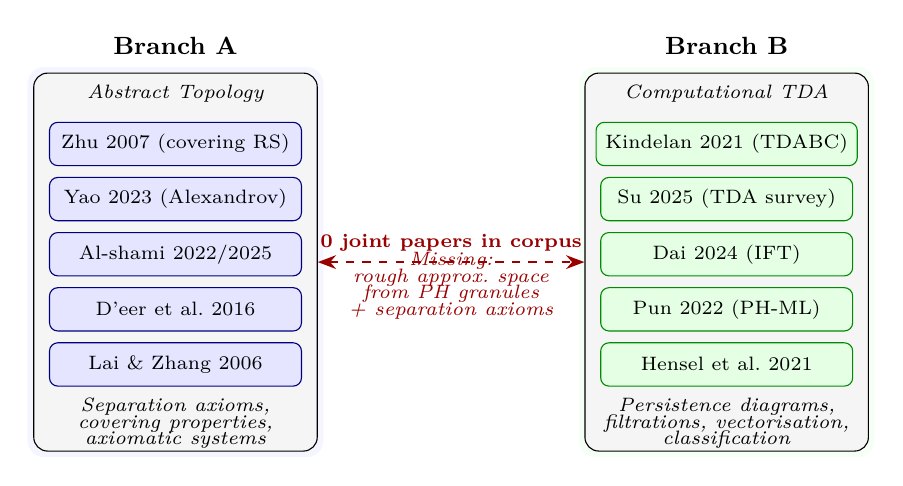
\begin{tikzpicture}[
  branchbox/.style = {draw, rounded corners=5pt, fill=gray!8,
                      minimum width=3.6cm, minimum height=4.8cm,
                      align=center},
  paper/.style     = {draw, rounded corners=3pt,
                      minimum width=3.2cm, minimum height=0.55cm,
                      align=center, font=\scriptsize, fill=white},
  paperA/.style    = {paper, fill=blue!10,   draw=blue!50!black},
  paperB/.style    = {paper, fill=green!10,  draw=green!55!black},
  titlestyle/.style= {font=\small\bfseries},
  arr/.style       = {-{Stealth[length=4pt]}, thick},
  gaparr/.style    = {<->, >=Stealth, thick, dashed, red!60!black},
]

%% ── Branch A column ──────────────────────────────────────────────────────────
\node[branchbox] (boxA) at (0,0) {};
\node[titlestyle, above=3pt] at (boxA.north) {Branch A};
\node[font=\scriptsize\itshape, below=1pt] at (boxA.north) {Abstract Topology};

\node[paperA] (zA)  at (0, 1.5) {Zhu 2007 (covering RS)};
\node[paperA] (yA)  at (0, 0.8) {Yao 2023 (Alexandrov)};
\node[paperA] (aA)  at (0, 0.1) {Al-shami 2022/2025};
\node[paperA] (dA)  at (0,-0.6) {D'eer et al.\ 2016};
\node[paperA] (lA)  at (0,-1.3) {Lai \& Zhang 2006};

\node[font=\scriptsize, align=center] at (0,-2.05)
  {\textit{Separation axioms,}\\[-2pt]\textit{covering properties,}\\[-2pt]\textit{axiomatic systems}};

%% ── Branch B column  (x = 7.0, gap = 3.4 cm) ────────────────────────────────
\node[branchbox] (boxB) at (7.0,0) {};
\node[titlestyle, above=3pt] at (boxB.north) {Branch B};
\node[font=\scriptsize\itshape, below=1pt] at (boxB.north) {Computational TDA};

\node[paperB] (kB)  at (7.0, 1.5) {Kindelan 2021 (TDABC)};
\node[paperB] (sB)  at (7.0, 0.8) {Su 2025 (TDA survey)};
\node[paperB] (dB)  at (7.0, 0.1) {Dai 2024 (IFT)};
\node[paperB] (pB)  at (7.0,-0.6) {Pun 2022 (PH-ML)};
\node[paperB] (hB)  at (7.0,-1.3) {Hensel et al.\ 2021};

\node[font=\scriptsize, align=center] at (7.0,-2.05)
  {\textit{Persistence diagrams,}\\[-2pt]\textit{filtrations, vectorisation,}\\[-2pt]\textit{classification}};

%% ── Zero-link zone in between  (centre of gap = 3.5) ────────────────────────
\draw[gaparr] (boxA.east) -- node[above, font=\scriptsize\bfseries, red!60!black]
  {0 joint papers in corpus} (boxB.west);

\node[font=\scriptsize, align=center, text=red!60!black]
  at (3.5,-0.3) {\textit{Missing:}\\[-2pt]\textit{rough approx.\ space}\\[-2pt]\textit{from PH granules}\\[-2pt]\textit{+ separation axioms}};

%% ── Background shading ───────────────────────────────────────────────────────
\begin{scope}[on background layer]
  \node[fill=blue!4, rounded corners=6pt,
        fit=(boxA), inner sep=2pt] {};
  \node[fill=green!4, rounded corners=6pt,
        fit=(boxB), inner sep=2pt] {};
\end{scope}

\end{tikzpicture}
\caption{The two topology branches in this survey are not connected by any
paper in our corpus (Appendix~\ref{app:search}; retrieved September 2025).
Branch~A (abstract topology) establishes which algebraic
axioms GrC approximation spaces satisfy; Branch~B (computational TDA) uses
persistent homology for data analysis.  The gap is the missing theorem that
connects persistence-based granules to separation axioms --- an open problem
identified in Section~\ref{sec:open}.}
\label{fig:topo_gap}
\end{figure}

This gap is not merely bibliographic.  Branch~A shows that covering axioms
constrain which concepts can be exactly approximated; Branch~B provides a
data-driven mechanism for building coverings from geometric-topological
summaries.  A paper connecting the two---showing, for example, that
persistent-homological granules satisfy a T$_1$ or T$_2$ separation axiom
under certain dataset conditions---would be a new result.

However, Pattern~A warns that such a connection must be checked carefully:
the star operator in a Vietoris--Rips complex at scale $\varepsilon$ is,
for finite point clouds, equivalent to the fixed-radius ball neighbourhood
$\NB{}^\varepsilon$ when restricted to the input points.  A naive connection
reduces to NRS.  The contribution must come from using the \emph{persistent
filtration}---the birth/death structure across scales---rather than any
single scale.

\paragraph{Practical guidance.}
Any researcher wishing to bridge Branch~A and Branch~B should:
(i) define the persistence-based granule explicitly and check
    against Definitions~\ref{def:nb}--\ref{def:dep};
(ii) apply the Pattern~A diagnostic (Section~\ref{sec:patA}): does the
     granule at a fixed filtration scale reduce to $\delta$-ball NRS?  If
     yes, the contribution must derive from the multi-scale structure;
(iii) verify experimentally that the resulting reduct is smaller or its
     boundary region is smaller than GBNRS on the same benchmark (a high bar
     given GBNRS's 259 citations and well-tuned defaults).

\section{Axis 3: Computational Efficiency}
\label{sec:efficiency}

The computational bottleneck of neighbourhood rough sets is the dependency
evaluation $\DEP(B \cup \{a\})$ for each candidate attribute $a$ at each
forward-greedy step.  Na\"ively, this costs $O(n^2 d)$: for each of the
$n^2/2$ object pairs, check whether they share a neighbourhood granule
under $B$.  For large $n$ (thousands of objects) or large $d$ (gene expression),
this is prohibitive.  Three families of acceleration have emerged.

%-----------------------------------------------------------------------
\subsection{Object-Pair Acceleration}
\label{sec:pair_accel}
%-----------------------------------------------------------------------

\paragraph{Maximal discernibility pairs (Dai et al., 2018).}
Rather than maintaining a dependency degree over all $n^2/2$ pairs, Dai et
al.~\cite{Dai2018TFS} observe that once a pair $(x_i, x_j)$ has been
\emph{discerned} by the current attribute subset $B$ (i.e., they fall in
different neighbourhoods), it does not need to be revisited when adding
further attributes.  The working set of pairs shrinks monotonically as $B$
grows.  This yields the concept of \emph{reduced maximal discernibility
pairs}: the minimal set of cross-class object pairs sufficient to determine
which attributes can further increase $\DEP$.  Empirically, the working set
reaches $\leq 20\%$ of all pairs on typical UCI datasets.

\paragraph{Parallel discernibility matrix (Sowkuntla \& Prasad Rao, 2021).}
The discernibility matrix representation of a fuzzy rough set---one row per
cross-class pair, one column per attribute---is sparser than the full
similarity matrix and decomposes naturally across rows.
Sowkuntla and Prasad Rao~\cite{Sowkuntla2021DARA} implement this decomposition
via MapReduce, reporting linear speedup on large datasets.  The key observation---discernibility
matrix rows are cheaper and more parallelisable than similarity matrix rows---was
identified independently but shares its core argument with Dai et al.'s
working-set reduction.

\paragraph{Discernibility hashing (Luo et al., 2025).}
Luo et al.~\cite{Luo2025hash} further compress the discernibility matrix by
hashing each row's attribute support set into a fixed-size hash space.
Two rows with the same support hash to the same bucket; only canonical
representatives per bucket are processed.  This reduces the effective matrix
size from $O(n^2)$ rows to $O(H)$ buckets (where $H$ is the hash table size),
with controllable collision probability.

%-----------------------------------------------------------------------
\subsection{Feature-Space Acceleration}
\label{sec:feat_accel}
%-----------------------------------------------------------------------

\paragraph{Grouping + representative selection.}
A complementary strategy groups attributes by mutual redundancy (clustering in
feature space) and selects one representative per group.  Kuzudisli et
al.~\cite{Kuzudisli2023review} survey this family, which encompasses FCBF
(Yu \& Liu~\cite{YuLiu2004}, 2321 citations), graph-based grouping
(Zheng et al.~\cite{Zheng2021grouping}; Wan et al.~\cite{Wan2023TFS}), and
cascaded fuzzy clustering (Chen et al.~\cite{Chen2024cascade}).
The redundancy within each group can be formalised in granular terms:
two attributes $a, b$ are \emph{granularly redundant} if
$\NB{\{a\}}(x) = \NB{\{b\}}(x)$ for all $x$; the granule geometry is then
a natural basis for the clustering step.

%-----------------------------------------------------------------------
\subsection{Distance Concentration as a Barrier}
\label{sec:concentration}
%-----------------------------------------------------------------------

All pair-pruning strategies share a vulnerability at high dimension:
\emph{concentration of measure}.  In $d$-dimensional space, the ratio
$(\max_{i,j} \rho(x_i,x_j)) / (\min_{i,j} \rho(x_i,x_j)) \to 1$ as
$d \to \infty$ for many distributions.  When all distances are nearly equal,
pruning by triangle inequality (``if $\rho(a,c) > \rho(a,b) + \rho(b,c)$
then prune'') offers no saving because no triangle inequality is violated.
Song et al.'s TRIM~\cite{TRIM2025} showed in the vector-search context that
pruning ratios collapse to near-zero at $d > 100$ without landmark-based
corrections.

The same barrier applies to rough set pair acceleration at high $d$.
The literature benchmarks primarily on $d \leq 60$ (Sonar, Ionosphere);
GBNRS reports results on up to $d = 166$ (Musk1).  Whether any of these
acceleration techniques survive at $d \sim 10^3$ (genomics) is unknown
and constitutes an open problem (Section~\ref{sec:open}).

\section{Axis 4: Sufficiency and Limits}
\label{sec:sufficiency}

The fourth axis concerns what a reduct \emph{cannot} guarantee.  Granular
computing finds a subset $R \subseteq \C$ that preserves the dependency
degree $\DEP(R) = \DEP(\C)$---but $\DEP(\C)$ itself may be far from 1.
Understanding the ceiling of what feature selection can achieve requires
results from classical learning theory that the GrC literature rarely cites.

%-----------------------------------------------------------------------
\subsection{Bayes Error Lower Bound}
\label{sec:bayes}
%-----------------------------------------------------------------------

The \emph{Bayes error} $R^* = \inf_f \mathbb{P}[f(X) \neq Y]$ is the
minimum achievable classification error over all measurable functions.
No feature set $R$, however well chosen, can reduce the empirical error
below $R^*$.

Cover and Hart~\cite{CoverHart1967} proved that the 1-NN rule achieves
error $R \leq R^*(2 - |\mathcal{D}|R^*/(|\mathcal{D}|-1))$ as $n\to\infty$;
in the binary case, $R \leq 2R^*(1-R^*)$, so $R \leq 2R^*$.  This result
implies that if a dataset has high inherent class overlap (high $R^*$), a
$k$-NN classifier on the reduct cannot do much better than twice the Bayes
error.

For finite samples, Drakopoulos~\cite{Drakopoulos1995} derives bounds on
classification error of the NN rule as a function of sample size and the
H\"older continuity of the class-conditional densities.  Wheat et
al.~\cite{Wheat2025BER} report Monte Carlo experiments showing that
practical BER estimators require at least 1000 samples per class to achieve
a 95\% confidence interval narrower than 5\%, and that accuracy degrades
rapidly as $d$ grows---a further endorsement of the concentration barrier
discussed in Section~\ref{sec:concentration}.

\paragraph{Implication for the dependency degree.}
When $\DEP(\C) < 1$, the dataset has a non-empty boundary region: some
objects are inherently ambiguous.  A reduct preserving $\DEP$ preserves
this ambiguity.  At a fixed radius $\delta$, $\DEP(\C)$ gives the fraction of training objects
whose neighbourhood falls entirely within one class (at that $\delta$); the remaining
$1-\DEP(\C)$ (boundary region) cannot be deterministically resolved by any
reduct at that $\delta$.  Unlike $R^*$, which is a population quantity,
$\DEP(\C)$ is an in-sample, $\delta$-dependent statistic: as $\delta\to 0$,
every granule becomes a singleton and $\DEP \to 1$, so $\DEP$ alone does not
bound generalisation error.  Accuracy on boundary objects is further
constrained by $R^*$.  The pair $(1-\DEP(\C),\,R^*)$ brackets the difficulty
of reduct-based classification from two complementary angles (in-sample
ambiguity and population-level irreducibility), yet the rough set literature
rarely reports or estimates either.

%-----------------------------------------------------------------------
\subsection{Class Overlap and Dataset Hardness}
\label{sec:overlap}
%-----------------------------------------------------------------------

Santos et al.~\cite{Santos2022overlap} provide a unified taxonomy of class
overlap measures, arguing that overlap (not imbalance per se) is the primary
driver of classification difficulty.  Their taxonomy distinguishes:
(a) \emph{feature overlap}: class conditional distributions share support;
(b) \emph{borderline overlap}: classes are locally mixed near the decision
boundary; (c) \emph{rare case overlap}: a few minority instances fall deep
in the majority region.

Han et al.~\cite{Han2024MFII} propose MFII, a complexity measure that
quantifies the joint effect of skewed distribution, overlap size, confusion
degree, and sub-cluster structure.  They also define ``value of
resolution'' (VoR) and ``degree of consistency'' (DoC) to evaluate whether
a complexity measure is discriminating: a measure with low VoR cannot
distinguish between datasets that respond differently to the same classifier.

The boundary region $\mathrm{BND}_R(d) = \UPP_R(d) \setminus \LOW_R(d)$
is a natural rough-set measure of class overlap.  The connection between
$|\mathrm{BND}_R(d)|/|\U| = 1 - \DEP(R)$ and the Santos--Han complexity
taxonomy has not been formalised.  Such a connection would allow GrC
practitioners to anticipate, before running reduction, whether a reduct
is likely to help or whether the dataset is in a regime where all methods
are near-optimal (i.e., near $R^*$).

%-----------------------------------------------------------------------
\subsection{Indirect and Weak Supervision}
\label{sec:weak}
%-----------------------------------------------------------------------

A reduct requires labelled training data to evaluate $\DEP(B)$.  Much
practical data arrives with indirect, noisy, or aggregate labels.

\paragraph{Learning from label proportions (LLP).}
In LLP, the learner observes only the class proportion within groups of
objects, not individual labels.  PAC-style analyses of LLP (see the survey by
Zhang et al.~\cite{Zhang2022PWS}, Section~4) suggest that learning requires
$O(1/\varepsilon^2)$ groups of size $O(\log(1/\delta))$ for
$(\varepsilon,\delta)$-accuracy; the sample complexity grows with the number
of classes but remains polynomially manageable.
A GrC-specific open problem is whether the dependency degree $\DEP(B)$
computed on aggregate label proportions converges to the clean-label
dependency degree as group size grows.

\paragraph{Partial label learning (PLL).}
In PLL, each object is annotated with a \emph{candidate set} of labels,
exactly one of which is correct.  Qian et al.~\cite{Qian2023InfoFusion}
combine granular ball computing with NRS to disambiguate candidate labels
before computing feature significance; their method adapts the rough set
reduct pipeline to the PLL setting with competitive accuracy on eight
benchmark datasets.  Wang et al.~\cite{Wang2018TNNLS} address the case
where some fraction of labels is randomly corrupted (not merely ambiguous),
providing an importance-reweighting strategy and consistency guarantees.

\paragraph{Programmatic weak supervision.}
Zhang et al.~\cite{Zhang2022PWS} survey programmatic weak supervision
(PWS), where labelling functions replace manual annotation.  The label model
in PWS estimates the accuracy of each labelling function; the resulting
probabilistic labels could, in principle, be used as a soft version of $d$
for computing $\DEP$.  This connection has not been explored in the GrC
literature.

\paragraph{Conformal prediction.}
Conformal prediction~\cite{Angelopoulos2023CP} provides finite-sample,
distribution-free prediction sets containing the true label with a
user-specified probability $1-\alpha$, without model or distributional
assumptions.  The positive region $\POS_R(d)$ offers a natural analogue: objects
in $\POS_R(d)$ receive singleton predictions (certain class membership) while
boundary objects are assigned multi-label sets.  This correspondence suggests
that reduct-based classification is implicitly performing a form of conformal
prediction with the nonconformity score defined by the neighbourhood
dependency.  Formalising this connection---including whether the positive-region coverage
provides distribution-free guarantees analogous to conformal prediction's
marginal coverage bound---has not been explored in the GrC literature.

\paragraph{Assessment of the sufficiency axis.}
The boundary between ``insufficient supervision'' and ``low dependency
degree'' is conceptually tight but notationally separate in the two
literatures.  A rough set reduct computed on noisy labels has a lower
$\DEP$ than the same reduct computed on clean labels; the gap between these
two $\DEP$ values is a natural measure of labelling noise.  This
interpretation is implicit in VPGB~\cite{Peng2022VPGB} and Qian et
al.~\cite{Qian2023InfoFusion} but has not been stated as a theorem.

Table~\ref{tab:sufficiency_synth} synthesises the four frameworks of this
section, showing what each bounds, whether GrC uses it, and where the gap
lies.

\begin{table*}[pos=!htbp]
\caption{Synthesis of sufficiency frameworks: what each bounds, its current
use in GrC, and the open gap.}
\label{tab:sufficiency_synth}
\centering\small
\begin{tabular}{p{3.0cm}p{3.8cm}p{3.0cm}p{4.5cm}}
\toprule
Framework & What it bounds & GrC adoption & Open gap \\
\midrule
Bayes error ($R^*$)
  & Population-level irreducible error
  & Rarely estimated; $\DEP$ used as proxy
  & Mapping $R^*$ to optimal purity $\tau$ (OP1) \\
\addlinespace
Class overlap (Santos--Han)
  & Dataset-level feature/border/rare-case overlap
  & Not connected to $\mathrm{BND}_R(d)$
  & Formal link between overlap profile and boundary region \\
\addlinespace
Weak/partial supervision
  & Label quality $\to$ $\DEP$ degradation
  & Implicit in VPGB, PLL-GBNRS
  & Tight bound on $|\DEP^* - \DEP^\eta|$ as function of noise rate (OP5) \\
\addlinespace
Conformal prediction
  & Marginal coverage at confidence $1{-}\alpha$
  & Not used in GrC
  & Whether POS coverage provides distribution-free guarantees \\
\bottomrule
\end{tabular}
\end{table*}

\section{Three Recurring Failure Patterns}
\label{sec:failure}

Across the four axes surveyed in Sections~\ref{sec:geometry}--\ref{sec:sufficiency},
and through our own experimental programme, we identify three structural reasons
why importing a modern mathematical framework into granular computing's core
pipeline tends not to produce a publishable contribution---or produces one that
does not stand up to independent scrutiny.  We call these \emph{Pattern~A}
(reduction to a known quantity), \emph{Pattern~B} (dominance of
label-orthogonal geometry),
and \emph{Pattern~C} (self-optimising evaluation); Figure~\ref{fig:patterns}
maps each pattern to the stage of the GrC pipeline where it arises.
They are not mutually exclusive; a single proposal can exhibit all three.
Section~\ref{sec:trends} shows how three current research directions
(incremental selection, three-way decision, neural-augmented GrC) can
navigate these patterns when evaluated correctly.

%-----------------------------------------------------------------------
\subsection{Pattern A: Reduction to a Known Granular Quantity}
\label{sec:patA}
%-----------------------------------------------------------------------

The most common failure is definitional: once the new quantity is unfolded,
it coincides with---or is bounded trivially by---a quantity already present
in the granular computing literature.

\paragraph{Example~A1: H$_0$ persistence and single-linkage clustering.}
The zero-dimensional persistent homology diagram of a point cloud under a
Vietoris--Rips filtration records the birth and death of connected components.
The death of a component at scale $\varepsilon$ marks the moment two
components merge---exactly the linkage event in single-linkage hierarchical
clustering.  This correspondence is a standard result: the $H_0$ barcode
of a Vietoris--Rips filtration is the merge tree of single-linkage
clustering, equivalently the minimum spanning tree's edge
weights~\cite{CarlssonMemoli2010hierarchical,Chazal2013persistenceclustering}.
Consequently, any attribute-importance score derived from the
H$_0$ diagram on the full feature set encodes the same information as the
single-linkage dendrogram, a quantity studied since the 1960s and available
in $O(n^2)$ time.  Example~A1 is therefore a genuine reduction, not an
analogy: the two quantities are equal, not merely correlated.

\paragraph{Example~A2: Supervised separation persistence and positive region.}
Consider a nearest-enemy superlevel filtration: each object $x$ is
``safe'' at radius $t$ if its nearest enemy is at distance $\geq t$;
connected components of safe objects form $H_0$ features as $t$ decreases.
Let $\phi(B)$ be the total persistence of these components under $B$.
An attribute is important if removing it reduces $\phi$.  After algebraic
simplification, the dominant term in $\phi(B)$ tracks the radius at which
class cores first connect to an enemy---that is, $1 - \DEP(B)$, where
$\DEP(B) = |\POS_B(d)|/|\U|$ is the NRS dependency degree at the same
radius.  The residual terms encode within-class boundary complexity, but
in the standard NRS regime where class cores are the dominant signal,
supervised persistence and NRS dependency convey the same ranking
information.  We state this as a heuristic reduction rather than an
identity: unlike Example~A1 we have no proof that the residual terms are
uninformative, only the observation that they vanish when every class core
is separated from its nearest enemy by a single scale.  The weaker claim is
enough for the diagnostic purpose---a proposal in this shape carries the
burden of showing that its residual is not negligible---but it is not
enough to assert equality, and we do not.

\paragraph{Example~A3: Fuzzy-T2 discernibility profiles and maximal
discernibility pairs.}
The proposal to use a fuzzy T$_2$ (Hausdorff-separation) degree between
attribute \emph{profiles}---vectors $\Delta_a(i,i') = |a(x_i)-a(x_{i'})|$
over cross-class pairs---as a basis for partitioning attributes shares its
core insight with Dai et al.~\cite{Dai2018TFS}: algorithms that operate on
object pairs can ignore already-discerned pairs, reducing cost from $O(m \cdot n^2)$
to $O(m\cdot|D|)$ where $D$ is the active discernibility set.
The T$_2$ framing adds topological language without adding
computational or theoretical content beyond that 176-cited result.

\paragraph{Diagnostic.}
Pattern~A is diagnosable before any experiment: write out the new quantity
symbolically and ask whether it is a monotone transformation of an existing
granular measure.  If the Jacobian of the mapping is bounded and non-vanishing,
the two quantities carry the same information up to a scaling factor.

%-----------------------------------------------------------------------
\subsection{Pattern B: Dominance of Label-Orthogonal Geometry}
\label{sec:patB}
%-----------------------------------------------------------------------

The second failure arises when the new importance signal is dominated by
properties of a feature's distribution that carry no information about the
decision task.  Measurement scale is the most familiar such property and the
one a stability bound like Theorem~\ref{thm:pai_bound} makes explicit, so we
begin there---but, as the evidence below shows, it is a special case rather
than the whole pattern, and a proposal can fail this way while surviving a
scale check.

\paragraph{Experimental evidence.}
We computed persistence-based attribute importance (PAI)---bottleneck distance
between the full persistence diagram and the diagram after removing attribute
$j$---on ten UCI datasets.  Each of five seeds draws one 80\% subsample without
replacement, giving five importance vectors per method and dataset
(total: $4{,}975$ measurements; raw data released as
\texttt{raw\_importance.csv}).  Downstream accuracies are separate: they come
from stratified 5-fold cross-validation repeated over the same five seeds,
with every importance ranking recomputed inside each training fold
(Section~\ref{sec:protocol}).
Table~\ref{tab:iris_top} reports the top-ranked attribute by PAI and by NRS
dependency on the Iris dataset as a representative example.

% AUTO-GENERATED by gen_tables.py -- do not edit by hand.
% Regenerate:  python3 gen_tables.py   Audit:  python3 verify_tables.py
\begin{table}[pos=!htbp]
\caption{Top-ranked attribute by method on Iris ($n=150$, $d=4$).  The
top-1 attribute is the arg-max of mean importance over the five seed
subsamples; the accuracies are mean $\pm$ SD over the 25 cross-validation
runs (5 folds $\times$ 5 seeds) using only that attribute. PAI
selects the attribute whose removal most disrupts the persistence diagram;
NRS selects the most discriminative attribute for the class label.}
\label{tab:iris_top}
\centering\small
\begin{tabular}{lccc}
\toprule
Method & Top-1 attribute & 3-NN acc.\ (top-1) & SVM acc.\ (top-1) \\
\midrule
PAI  & \texttt{sepal\_width}  & $48.9 \pm 7.4$\% & $54.0 \pm 8.4$\% \\
NRS  & \texttt{petal\_width}  & $95.9 \pm 3.9$\% & $96.0 \pm 3.5$\% \\
\bottomrule
\end{tabular}
\end{table}


PAI ranks \texttt{sepal\_width} first because removing it causes the largest
bottleneck-distance shift in the persistence diagram, even though it
contributes no class signal at the neighbourhood scale used by NRS.
\texttt{petal\_width}, the most discriminative attribute (NRS top-1),
receives a smaller PAI score because the persistence diagram is less
sensitive to its removal.
The downstream consequence is stark: selecting on PAI yields 3-NN accuracy of
48.9\% (barely above the 33\% three-class chance level) versus 95.9\%
for NRS.  The same pattern holds under SVM-RBF evaluation: PAI top-1 gives
54.0\% versus NRS top-1 at 96.0\%.

\paragraph{Generalisation across datasets.}
The Iris result is not an artefact of one dataset.
Table~\ref{tab:rho} reports the Spearman rank correlation $\rho$ between PAI
and NRS importance across all ten benchmarks.

% AUTO-GENERATED by gen_tables.py -- do not edit by hand.
% Regenerate:  python3 gen_tables.py   Audit:  python3 verify_tables.py
\begin{table}[pos=!htbp]
\caption{Spearman $\rho$ between PAI and NRS importance rankings per dataset
(mean importance over 5 seeds before ranking; $d$ = number of attributes,
which is also the sample size for the Spearman test).
Note: datasets with $d \leq 7$ cannot reach $p < 0.05$ at any $\rho$.}
\label{tab:rho}
\centering\small
\begin{tabular}{lccc}
\toprule
Dataset & $d$ & $\rho$ & $p$-value \\
\midrule
Iris       &  4 & $-0.80$ & $0.20$ \\
Wine       & 13 & $-0.29$ & $0.34$ \\
Ionosphere & 34 & $-0.17$ & $0.35$ \\
Sonar      & 60 & $+0.04$ & $0.76$ \\
Glass      &  9 & $+0.06$ & $0.88$ \\
Ecoli      &  7 & $+0.71$ & $0.07$ \\
Heart      & 13 & $+0.08$ & $0.79$ \\
Parkinsons & 22 & $+0.30$ & $0.17$ \\
Seeds      &  7 & $+0.21$ & $0.64$ \\
WDBC       & 30 & $-0.50$ & $0.01$ \\
\midrule
Mean (10)  & --- & $-0.034$ & --- \\
\bottomrule
\end{tabular}
\end{table}


Table~\ref{tab:rho} shows the ten-dataset picture.
The three-dataset pilot (Iris, Wine, Ionosphere) produced $\bar\rho=-0.42$,
suggesting complementarity.  The full run gives $\bar\rho = -0.034$, consistent
with zero correlation.  A Fisher-$z$ weighted aggregate (weights $d_i - 3$)
gives $\bar\rho_z = -0.060$, 95\% CI $[-0.207,\,+0.091]$, with
heterogeneity $Q = 15.8$, $I^2 = 43\%$---the confidence interval straddles
zero, confirming no systematic relationship.
Only one $\rho$ is individually significant
(WDBC, $d=30$, $\rho=-0.50$, $p=0.01$); on datasets with $d \leq 7$
(Iris, Ecoli, Seeds), the Spearman test has no power to reject the null
at any ranking.  Six rhos are positive, consistent with PAI and NRS ranking
attributes in the same order on more datasets than not, but a sign test on
6/10 is not significant ($p = 0.75$, two-sided binomial): the two methods are
uncorrelated, not complementary.  The pilot's apparent complementarity was not representative.

\paragraph{Classifier robustness (SVM-RBF).}
Following our own recommended practice (Section~\ref{sec:standard}), we
repeat the analysis with SVM-RBF ($C=1$, $\gamma=\text{scale}$), a
classifier whose geometry differs from the $k$-NN rule.  Over $k < d$,
mean SVM accuracy is: NRS $85.1\%$, PAI $80.2\%$ ($p = 0.006$, dataset-level
Wilcoxon, $n=10$; PAI wins on 1/10 datasets).  The SVM results confirm
the 3-NN finding: PAI's inferiority is not an artefact of the classifier.

PAI is also expensive.  It is $\sim 380\times$ slower than NRS: mean of per-dataset median reduct time
is 6.5\,s for PAI vs 0.017\,s for NRS (on the same single-threaded harness).
ReliefF (0.068\,s) and mutual information (0.014\,s) are also orders of
magnitude faster.  One anomaly: Sonar ($d=60$) reports PAI median time of
0.018\,s, comparable to NRS (0.034\,s), despite having the highest
dimensionality; this suggests a computation shortcut or caching effect at
that particular filtration setting that warrants further investigation.
The general cost is inherent: PAI requires a full Rips
persistence computation per attribute per subsample, with $O(n^3)$ worst-case
complexity.

\paragraph{Additional baselines: hybrid and null.}
The released data includes a hybrid ranking (\texttt{pai\_nrs}: the
element-wise mean of z-scored PAI and NRS importance vectors) and a variance
ranking (features ordered by sample variance on the z-scored data---effectively
a null baseline, since all variances centre near 1.0).  Neither rescues PAI.
Over $k < d$, mean 3-NN accuracy is: NRS $83.7\%$, PAI+NRS hybrid $80.1\%$
($p = 0.010$ vs NRS, Wilcoxon), PAI $77.6\%$ ($p = 0.004$ vs PAI+NRS).
The variance baseline achieves $79.0\%$---statistically indistinguishable
from PAI ($p = 0.23$).  That a null ranking matches PAI is the sharpest
available statement of the negative result.

\paragraph{Root cause: theoretical bound vs empirical behaviour.}
Theorem~\ref{thm:pai_bound} guarantees $\mathrm{PAI}(j) \leq \mathrm{range}(a_j)$:
the bound is proportional to the feature's range.  One might therefore
hypothesise that PAI scores track range, making them scale artefacts.
We test this directly.  Table~\ref{tab:pai_range} reports the Spearman
$\rho$ between PAI and $\mathrm{range}(a_j)$ per dataset on the z-scored
data actually used.

% AUTO-GENERATED by gen_tables.py -- do not edit by hand.
% Regenerate:  python3 gen_tables.py   Audit:  python3 verify_tables.py
\begin{table}[pos=!htbp]
\caption{Spearman $\rho$ between mean PAI score and
$\mathrm{range}(a_j)$ per dataset.  Data is z-score standardised,
so range variation across features reflects kurtosis and outlier
structure, not raw measurement scale.}
\label{tab:pai_range}
\centering\small
\begin{tabular}{lccc}
\toprule
Dataset & $d$ & $\rho(\text{PAI},\text{range})$ & $p$ \\
\midrule
Iris       &  4 & $+0.80$ & $0.200$ \\
Wine       & 13 & $+0.64$ & $0.019$ \\
Ionosphere & 34 & $+0.42$ & $0.014$ \\
Sonar      & 60 & $+0.33$ & $0.010$ \\
Glass      &  9 & $-0.52$ & $0.154$ \\
Ecoli      &  7 & $-0.54$ & $0.215$ \\
Heart      & 13 & $-0.04$ & $0.887$ \\
Parkinsons & 22 & $-0.85$ & $<0.001$ \\
Seeds      &  7 & $+0.89$ & $0.007$ \\
WDBC       & 30 & $+0.35$ & $0.060$ \\
\midrule
Mean (10)  & --- & $+0.15$ & --- \\
\bottomrule
\end{tabular}
\end{table}


The mean correlation is $+0.15$ and highly heterogeneous: Parkinsons is
\emph{significantly negative} ($\rho = -0.85$, $p < 0.001$).  The
theoretical bound of Theorem~\ref{thm:pai_bound} is far from tight
(mean ratio $0.038$, max $0.194$; equivalently $0.075$ and $0.387$ against
the sharper per-dimension bound), so range is not the \emph{primary} driver
of PAI on most datasets.  The
mechanism is subtler: PAI measures how much removing a coordinate
changes the \emph{global topology} of the point cloud, a quantity that
depends on the interaction between the coordinate's distribution (kurtosis,
outlier structure after z-scoring) and the dataset's geometric embedding.
This sensitivity to global geometry rather than local class structure is why
PAI fails as a supervised importance measure.

This is also why we define Pattern~B by label-orthogonality rather than by
scale.  Had we kept the narrower definition, our own flagship example would
not satisfy it: PAI's correlation with range is significantly positive on
only four of ten datasets and significantly \emph{negative} on one, so
``dominated by range'' is not what the data show.  What the data do show is
that PAI is computed entirely from the geometry of the unlabelled point
cloud, is uncorrelated with discriminability (Table~\ref{tab:rho}), and is
indistinguishable from a variance null baseline downstream ($p=0.23$).  The
failure is that the imported quantity measures something real about the data
that has no bearing on the decision; measurement scale is the instance of
that failure a stability theorem can bound, which is why it is the one the
literature notices.

Note that the data is z-score standardised (Section~\ref{sec:protocol}), so
all features have unit variance; the residual range variation comes from
kurtosis and outliers.  This makes the negative result stronger
than it would be on raw data: even after removing the obvious scale artefact
via standardisation, PAI still does not align with discriminative importance.

\paragraph{Generality.}
Pattern~B is not specific to persistent homology.  Any importance measure
$s_j$ that is computed from the geometry of the feature distribution without
reference to the label is at risk, and a bound depending on measurement-scale
properties of $a_j$ (range, variance, inter-quantile spread) is the visible
symptom rather than the disease.  For purely
distance-based importance (e.g.\ Relief, HSIC with Gaussian kernel), the
community has learned to z-score inputs before applying such methods.  The
PAI case shows that z-scoring is necessary but not sufficient: homological
stability introduces a dependency on the \emph{shape} of each coordinate's
distribution that standardisation does not remove.

%-----------------------------------------------------------------------
\subsection{Pattern C: Self-Optimising Evaluation}
\label{sec:patC}
%-----------------------------------------------------------------------

The third failure is evaluative: the new method is benchmarked against metrics
that are algebraically related to---or optimised by construction by---the
method's own objective.

\paragraph{Experimental evidence.}
We evaluated five feature-selection methods (PAI, NRS,
ReliefF~\cite{Kononenko1994,RobnikKononenko2003}, mutual information
(mRMR~\cite{Peng2005mRMR}), and variance) on structure-preservation metrics: Wasserstein distance
of persistence diagrams (\texttt{wass\_persist}), trustworthiness
(\texttt{trust}), $k$-NN overlap (\texttt{knn\_overlap}), and adjusted Rand
index of cluster structure (\texttt{cluster\_ari}).
Results across ten datasets are in Table~\ref{tab:structure}.

% AUTO-GENERATED by gen_tables.py -- do not edit by hand.
% Regenerate:  python3 gen_tables.py   Audit:  python3 verify_tables.py
\begin{table}[pos=!htbp]
\caption{Structure-preservation comparison, PAI vs NRS (10 datasets).
\texttt{wass\_persist} is lower-is-better (PAI's own metric); the others are
higher-is-better and are not algebraically tied to PAI's objective.  Note that
\texttt{trust} and \texttt{knn\_overlap} share a neighbourhood-size parameter,
fixed here at the conventional $K=10$ and ablated in
Table~\ref{tab:knn_scale}.  Means, SDs, win counts
and tests all use the same aggregation: one value per dataset, averaged over
$k<d$.  $p$-values: dataset-level paired Wilcoxon signed-rank
($n=10$, two-sided).}
\label{tab:structure}
\centering\small
\begin{tabular}{lcccc}
\toprule
Metric & PAI (mean $\pm$ SD) & NRS (mean $\pm$ SD) & PAI wins / 10 & $p$ \\
\midrule
\texttt{wass\_persist}  & $66.7 \pm 40.1$ & $77.4 \pm 51.2$ & 8/10 & $0.049$ \\
\texttt{knn\_overlap}   & $0.530 \pm 0.075$ & $0.474 \pm 0.090$ & 8/10 & $0.064$ \\
\texttt{trust}          & $0.889 \pm 0.024$ & $0.903 \pm 0.030$ & 1/10 & $0.006$ \\
\texttt{cluster\_ari}   & $0.482 \pm 0.122$ & $0.665 \pm 0.119$ & 1/10 & $0.004$ \\
\bottomrule
\end{tabular}
\end{table}


PAI wins on \texttt{wass\_persist} (8/10 datasets, $p=0.049$; lower is
better)---because PAI selects features that best preserve the persistence
diagram, precisely what Wasserstein distance measures.  This is the only
metric of the four on which PAI's advantage reaches significance, and it is
the one algebraically tied to PAI's objective.  PAI also scores higher on
\texttt{knn\_overlap} on 8/10 datasets, at $p=0.064$ under the default
neighbourhood size $K=10$.  Rather than explain this away, we tested it.

\paragraph{Is the \texttt{knn\_overlap} edge a scale artefact?  A direct test.}
The natural explanation is that PAI's bottleneck objective and $k$-NN overlap
probe the same local neighbourhoods, so the advantage should be largest when
$K$ matches the scale PAI's filtration actually sees and should decay as the
two are mismatched.  That explanation is post-hoc until tested, so we ran the
discriminating experiment: holding the selected feature subsets fixed at those
of Table~\ref{tab:structure}, we recomputed the metric for
$K \in \{3,5,10,20,30,50\}$.  Crucially we did the same for
\texttt{trust}, which takes the same neighbourhood parameter and is
also conventionally left at $K=10$---ablating only the metric that favours
PAI would repeat the selective reporting this survey criticises.
Table~\ref{tab:knn_scale} reports both.

% AUTO-GENERATED by gen_tables.py -- do not edit by hand.
% Regenerate:  python3 gen_tables.py   Audit:  python3 verify_tables.py
\begin{table}[pos=!htbp]
\caption{Ablation of the neighbourhood parameter $K$ shared by the two
local structure metrics.  Feature subsets are exactly those of
Table~\ref{tab:structure}; only $K$ changes.  Each row aggregates over $k<d$
per dataset, then compares PAI with NRS by dataset-level paired Wilcoxon
signed-rank ($n=10$, two-sided); $\Delta = \mathrm{PAI}-\mathrm{NRS}$, and
$^{*}$ marks $p<0.05$.  $K=10$ is the default used in
Table~\ref{tab:structure} and throughout the literature.}
\label{tab:knn_scale}
\centering\small
\begin{tabular}{cccccc}
\toprule
$K$ & PAI & NRS & $\Delta$ & PAI wins / 10 & $p$ \\
\midrule
\multicolumn{6}{l}{\emph{\texttt{knn\_overlap}} (higher is better)} \\
 3 & $0.407$ & $0.328$ & $+0.079$ & 8/10 & $0.037$\,$^{*}$ \\
 5 & $0.459$ & $0.387$ & $+0.072$ & 8/10 & $0.037$\,$^{*}$ \\
10 & $0.530$ & $0.474$ & $+0.056$ & 8/10 & $0.064$ \\
20 & $0.599$ & $0.570$ & $+0.029$ & 7/10 & $0.160$ \\
30 & $0.643$ & $0.628$ & $+0.014$ & 7/10 & $0.275$ \\
50 & $0.697$ & $0.710$ & $-0.013$ & 2/10 & $0.193$ \\
\addlinespace
\multicolumn{6}{l}{\emph{\texttt{trust}} (higher is better)} \\
 3 & $0.891$ & $0.904$ & $-0.012$ & 1/10 & $0.004$\,$^{*}$ \\
 5 & $0.890$ & $0.903$ & $-0.013$ & 1/10 & $0.004$\,$^{*}$ \\
10 & $0.889$ & $0.903$ & $-0.014$ & 1/10 & $0.006$\,$^{*}$ \\
20 & $0.889$ & $0.906$ & $-0.017$ & 1/10 & $0.004$\,$^{*}$ \\
30 & $0.890$ & $0.910$ & $-0.020$ & 1/10 & $0.004$\,$^{*}$ \\
50 & $0.890$ & $0.914$ & $-0.023$ & 1/10 & $0.004$\,$^{*}$ \\
\bottomrule
\end{tabular}
\end{table}


The advantage is entirely a small-$K$ phenomenon.  It is significant at
$K=3$ and $K=5$ ($p=0.037$), borderline at the default $K=10$ ($p=0.064$),
absent by $K=20$ ($p=0.16$), and at $K=50$ it reverses: PAI wins on
2/10 datasets and trails NRS by $0.013$.  An analyst who reports
\texttt{knn\_overlap} at $K=5$ concludes that PAI preserves neighbourhood
structure significantly better than NRS; an analyst who reports the same
metric at $K=50$ concludes the opposite, from the same feature subsets.  The
conclusion is determined by a free parameter of the evaluation metric.

The mechanism, however, is not the one we predicted.  If the advantage came
from a match between $K$ and PAI's own filtration scale, the $K$ maximising
the advantage would track that scale across datasets.  It does not.  Taking
the empirical filtration scale of each dataset to be the mean number of
points within the Rips threshold ($\varepsilon=2$ on standardised data), which
ranges from $1.6$ on Heart to $77.1$ on Ecoli, the rank correlation between
that scale and the advantage-maximising $K$ is $\rho=-0.10$ ($p=0.80$,
$n=9$ datasets with a non-degenerate scale); pooling all dataset--$K$ pairs,
the correlation between scale mismatch $|\log K - \log k_{\mathrm{PAI}}|$ and
the advantage is $\rho=-0.05$ ($p=0.74$).  Seven of ten datasets peak at
$K=3$ whether their filtration scale is $2$ or $77$.  We therefore withdraw
the same-neighbourhoods explanation: the edge is a generic small-$K$ effect,
not a signature of PAI's geometry.
(One dataset is degenerate in a way worth recording: on Sonar, $d=60$, no
point has \emph{any} neighbour within $\varepsilon=2$ after standardisation,
so PAI's filtration sees no connectivity at all---and Sonar is the one
dataset where PAI trails NRS at every $K$.)

The comparison with \texttt{trust} is what makes this conclusive.  That
metric carries the identical parameter, so if PAI's verdicts were generally
$K$-sensitive we should see it move too.  It does not move at all: PAI loses
on 1/10 datasets at every $K$ from 3 to 50, at $p \leq 0.006$ throughout, and
the gap widens with $K$ (from $-0.012$ at $K=3$ to $-0.023$ at
$K=50$).  The third metric, \texttt{cluster\_ari}, has no free local scale at
all---its cluster count is fixed to the number of classes---and agrees
($p=0.004$).

The asymmetry is the finding.  The metric on which PAI appears to lead is
precisely the one whose verdict an analyst selects when choosing $K$; the
metrics on which PAI loses return the same verdict at every setting of that
same parameter.  The negative result is therefore robust to the choice we
have just shown to be decisive elsewhere, and the apparent positive result is
not.  A paper that evaluates a
persistence-based selector only on persistence-based (or same-scale) downstream
metrics has demonstrated self-consistency, not generalisation.

\paragraph{Generality.}
Pattern~C recurs whenever evaluation and design share the same mathematical
object.  A coverage-based reduct evaluated by coverage, a mutual-information
selector evaluated by mutual information with the label, a graph-regularised
model evaluated by graph smoothness---all exhibit the same circularity.
The diagnostic is simple: if removing the proposed evaluation metric from the
paper would remove the only result where the method wins, Pattern~C is present.
A second form is subtler and, on the evidence of Table~\ref{tab:knn_scale}, at
least as common: if the metric carries a free parameter and the method's win
survives only in part of that parameter's range, the win is a property of the
parameter choice, not of the method.  Report the whole range, and check
whether the metrics that \emph{disagree} with the method are equally
sensitive---if they are not, that asymmetry is the result.

\paragraph{Recommended practice.}
For any proposed importance measure $s$, include at least one evaluation
metric $m$ such that $s \not\to \arg\max m$: that is, optimising $s$ does not
provably optimise $m$.  Downstream accuracy on held-out data with a classifier
that does not use $s$'s geometry (e.g., SVM-RBF or Random
Forest~\cite{Breiman2001RF} when $s$ is geometry-based)
serves this purpose if statistical significance is reported.

%-----------------------------------------------------------------------
\subsection{Diagnostic Checklist}
\label{sec:checklist}
%-----------------------------------------------------------------------

Before investing in implementation, a proposed GrC extension should pass
three checks:

\begin{enumerate}
\item \textbf{Anti-A}: Write the new quantity symbolically.  Is it a
monotone function of an existing granular quantity?  If yes, prove it is
strictly more informative, or abandon.
\item \textbf{Anti-B}: Is the quantity computed from the feature
distribution without reference to the label?  If so, standardisation is the
first test but not a sufficient one---our own experiments were run on
z-scored data and Pattern~B appeared regardless.  Run two checks, not one.
(i)~Correlate the score against a pure scale statistic (range, IQR) on the
standardised data; a significant positive correlation is a failure.
(ii)~More important, correlate it against an established
\emph{label-aware} importance measure: a score that is uncorrelated with
discriminability has failed even if it passes~(i), which is precisely what
PAI does (Table~\ref{tab:rho} versus Table~\ref{tab:pai_range}).  A
label-free geometric score must earn its place by predicting the label
better than a null ranking, not merely by being unlike range.
\item \textbf{Anti-C}: Identify at least one evaluation metric that is
not algebraically related to the method's objective.  Report that
metric as the primary result.
\end{enumerate}

These checks cost one afternoon; their absence costs months of wasted
implementation.

\section{Critique of Evaluation Practices}
\label{sec:methodology}

The three failure patterns of Section~\ref{sec:failure} are partly enabled
by a weak evaluation culture in the GrC feature-selection literature.
We document four recurring problems and propose minimum reporting standards.

%-----------------------------------------------------------------------
\subsection{The 3-NN/SVM-UCI Benchmark Is Insensitive}
\label{sec:insensitive}
%-----------------------------------------------------------------------

The dominant evaluation protocol in the field is: run forward-greedy
attribute reduction with a proposed significance measure; select the top-$k$
attributes; evaluate 3-NN or SVM-RBF on UCI datasets; report mean accuracy.
This protocol has a structural defect: on many UCI datasets, the baseline
of selecting \emph{all} features is competitive with or superior to the best
reduct---and that baseline is usually not reported, so the reader cannot see
the problem.  In the full-text coding of Table~\ref{tab:practice}, 17 of the
22 papers omit it---10 of the 13 that belong to our Axis-1 corpus.

Table~\ref{tab:allfeats} shows the best-$k$ accuracy achieved by any method
versus the all-features baseline on our ten-dataset benchmark.

% AUTO-GENERATED by gen_tables.py -- do not edit by hand.
% Regenerate:  python3 gen_tables.py   Audit:  python3 verify_tables.py
\begin{table}[pos=!htbp]
\caption{Best-$k$ 3-NN accuracy (maximised over methods and
$k \in \{1,\ldots,d\}$) versus all-features baseline.  Mean $\pm$ SD over
5~folds $\times$ 5~seeds.  $\Delta$ is the margin in percentage points;
$p_{\mathrm{Holm}}$ is a paired Wilcoxon signed-rank test over the 25
matched fold--seed pairs, Holm-corrected for the ten comparisons.
$\dagger$ marks the dataset where best-$k = d$, i.e.\ no strict subset
outperforms the full feature set.}
\label{tab:allfeats}
\centering\small
\setlength\tabcolsep{4pt}
\begin{tabular}{lrrccrrr}
\toprule
Dataset & $n$ & $d$ & All-feat acc. & Best-$k$ acc. & $k^*$ & $\Delta$ (pp) & $p_{\mathrm{Holm}}$ \\
\midrule
Iris       & 150 &  4 & $94.4 \pm 4.9$\% & $96.1 \pm 3.9$\% & 3 & $+1.73$ & $0.078$ \\
Wine       & 178 & 13 & $96.0 \pm 2.8$\% & $97.3 \pm 2.8$\% & 9 & $+1.35$ & $0.167$ \\
Ionosphere & 351 & 34 & $84.9 \pm 3.9$\% & $90.4 \pm 3.9$\% & 5 & $+5.48$ & $<0.001$ \\
Sonar      & 208 & 60 & $84.2 \pm 6.8$\% & $84.7 \pm 7.1$\% & 38 & $+0.47$ & $1.000$ \\
Glass      & 214 &  9 & $68.5 \pm 5.5$\% & $73.4 \pm 6.1$\% & 7 & $+4.85$ & $0.005$ \\
Ecoli      & 336 &  7 & $84.5 \pm 3.7$\% & $84.6 \pm 3.6$\% & 6 & $+0.06$ & $1.000$ \\
Heart      & 270 & 13 & $81.5 \pm 5.1$\% & $81.5 \pm 5.1$\% & 13$\dagger$ & $+0.00$ & $1.000$ \\
Parkinsons & 195 & 22 & $91.4 \pm 3.6$\% & $93.4 \pm 3.9$\% & 15 & $+2.05$ & $0.006$ \\
Seeds      & 210 &  7 & $92.5 \pm 3.6$\% & $93.1 \pm 3.3$\% & 4 & $+0.67$ & $1.000$ \\
WDBC       & 569 & 30 & $96.6 \pm 1.5$\% & $97.0 \pm 1.3$\% & 16 & $+0.46$ & $0.911$ \\
\bottomrule
\end{tabular}
\end{table}


The margins are small: seven of the ten datasets gain at most $2$ pp from
the best reduct over the whole feature set, and on Heart the best reduct
is the whole feature set.  Rather than declare a noise threshold by
inspection, we test each margin.  A paired Wilcoxon signed-rank test over the
25 matched fold--seed pairs, Holm-corrected for the ten comparisons, finds
the gain significant on only three datasets: Ionosphere ($+5.5$ pp),
Glass ($+4.9$ pp) and Parkinsons ($+2.1$ pp).  On the remaining seven the
best reduct that any of the seven methods can produce is statistically
indistinguishable from using every feature.
Figure~\ref{fig:margin} visualises the margins with this distinction.

The consequence for the field is the important part.  If the best
selector at the best $k$ cannot separate itself from the do-nothing
baseline on seven of ten standard benchmarks, then a comparison between two
selectors on those benchmarks is being conducted inside the interval where
the benchmark has no resolving power.  This is a property of the evaluation
protocol, not of any particular method, and it applies equally to our own
PAI results in Section~\ref{sec:failure}: the PAI-versus-NRS gaps we report
are large enough to survive it, but many published gaps are not.

\begin{figure}[pos=!htbp]
\centering
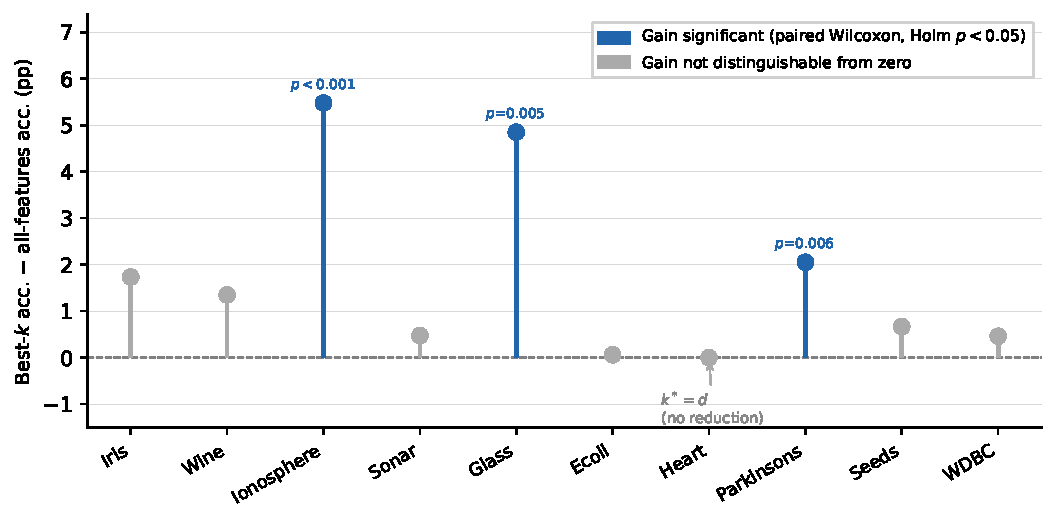
\includegraphics[width=\columnwidth]{figures/margin_plot.pdf}
\caption{Best-$k$ 3-NN accuracy minus the all-features baseline per
dataset (lollipop chart).  Blue: the gain is significant under a paired
Wilcoxon signed-rank test over the 25 matched fold--seed pairs after Holm
correction for the ten comparisons ($p<0.05$, value annotated); grey: the
gain is not distinguishable from zero.  Seven of ten datasets are grey,
so between-method comparisons at this benchmark scale are largely
uninformative.}
\label{fig:margin}
\end{figure}

%-----------------------------------------------------------------------
\subsection{Significance Testing Is Rare}
\label{sec:significance}
%-----------------------------------------------------------------------

Statistical testing is rare in the GrC feature-selection literature.
Zhang et al.~\cite{Zhang2023GiniNRS} state in their own paper---which proposes
a Gini-enhanced NRS variant and reports improvements on 16 UCI
datasets---that ``\emph{statistical tests reveal no significant differences
between the proposed algorithm and the four classical neighborhood rough
set-based feature selection algorithms}.''  The paper is published as an
improvement regardless.  This is not an isolated case: it reflects the
community's structural tolerance for non-significant comparisons on
low-sensitivity benchmarks.

\paragraph{How common is this?  A full-text coding.}
Answering this requires reading experimental sections, not abstracts.  We
read 22 attribute-reduction papers at full text and coded four
presence/absence facts from each paper's experimental section.  Thirteen of
them are members of this survey's Axis-1 corpus, and they are 13 of the 25
Axis-1 papers---so for the axis that dominates recent output
(Figure~\ref{fig:activity}) this is a majority coding, not an anecdote.
Table~\ref{tab:practice} reports the counts for both groupings, and
Table~\ref{tab:practice_detail} gives the per-paper judgements for the
corpus members.

% AUTO-GENERATED by gen_tables.py -- do not edit by hand.
% Regenerate:  python3 gen_tables.py   Audit:  python3 verify_tables.py
\begin{table}[pos=!htbp]
\caption{Reporting practice in attribute-reduction papers read at full text.
Each cell is a presence/absence judgement made from the experimental section
only; the coding and the supporting quotation for every cell are released as
\texttt{fulltext\_coding.csv}.  Column~2 covers all 22 papers
coded; column~3 restricts to the 13 that are members of this
survey's Axis-1 corpus (Appendix~\ref{app:search}), i.e.\ 13
of the 25 Axis-1 papers.}
\label{tab:practice}
\centering\small
\begin{tabular}{lcc}
\toprule
Practice & All coded ($n=22$) & Axis-1 corpus ($n=13$) \\
\midrule
All-features baseline reported & 5/22 & 3/13 \\
Dispersion (SD or per-fold) reported & 6/22 & 2/13 \\
Statistical significance test run & 12/22 & 7/13 \\
Own hyperparameter ablated & 7/22 & 3/13 \\
\midrule
\textbf{All four} & 0/22 & 0/13 \\
\textbf{None of the four} & 5/22 & 3/13 \\
\bottomrule
\end{tabular}
\end{table}


Within the Axis-1 corpus, 10 of 13 papers report no all-features baseline, so
a reader cannot tell whether selection helped at all; 11 of 13 report no
dispersion, so no reader can run the paired test the paper omitted; and 10 of
13 vary no hyperparameter of their own method.  Seven of 13 run a
significance test.  Three papers report none of the four practices.  Across all 22 papers
coded, \emph{not one reports all four}.

The single most consequential gap is the missing baseline.  Section~\ref{sec:insensitive}
showed that on seven of ten benchmarks the best reduct any method can produce
is statistically indistinguishable from keeping every feature.  A paper that
does not report the all-features number cannot detect that it is in this
regime, and neither can its reviewer.

\paragraph{What this coding can and cannot support.}
We state the limits precisely, because the alternative is the error this
section criticises.  The papers are those we could obtain in full text, not a
random draw, and they concentrate in the granular-ball and fuzzy-neighbourhood
branch: the Axis-1 figures generalise to Axis~1, not to Axes~2--4, which we do
not claim to have coded.  Counts are reported as fractions rather than
percentages of the field.  The coding records only whether a practice is
present, not whether it was done well---a paper credited with a significance
test may still have applied an inappropriate one, and one paper's test is run
on runtime rather than accuracy.  Judgements are deliberately conservative:
a mention of the ``original dataset'' in a method description or a figure
caption is not counted as a baseline, and tuning a comparison classifier's
$k$ is not counted as ablating one's own hyperparameter.  Every cell carries
the quotation it rests on, so an individual judgement can be overturned
without re-reading the paper.

A broader pattern is visible from our own evaluation: a 3-NN accuracy
difference of 1\% on a dataset of $n \leq 300$ objects corresponds to a
shift of 2--3 objects between folds, which is within the variance of a
single run.  Reporting means without standard deviations, and means without
a paired test across datasets, provides no evidence that a measured difference
exceeds noise.  Feature selection reviews in the ML literature~\cite{Saeys2007}
document the same insensitivity: no single filter or wrapper method dominates
across UCI benchmarks, and small-sample variance is the primary confound.

\paragraph{Minimum standard.}
Any claim of superiority over a baseline requires:
(a) per-fold accuracy (not just means), so a paired test is possible;
(b) a paired Wilcoxon signed-rank test across datasets or folds;
(c) effect size ($|\Delta \text{acc}|$, not just $p < 0.05$).

%-----------------------------------------------------------------------
\subsection{No Ablation of Generator Parameters}
\label{sec:ablation}
%-----------------------------------------------------------------------

GBNRS-family methods have one key hyperparameter: purity threshold $\tau$
(default $2/3$).  NRS methods have radius $\delta$.  Persistence-based
methods have filtration maximum $\varepsilon_{\max}$ and maximum homological
dimension $d_{\max}$.  Ablation of these is rare: in the full-text coding of
Table~\ref{tab:practice}, 15 of 22 papers vary no hyperparameter of their own
method, several stating a fixed value in passing---``the purity is set to
1''---without reporting what happens at any other setting.  The exceptions
show it is neither hard nor expensive: one sweeps the purity threshold from
$0.54$ to $1.0$ in fixed steps, another reports results for
$K \in \{1,\ldots,7\}$, and a third devotes a subsection to parameter
sensitivity.

Without ablation, it is impossible to determine whether an observed
improvement is due to the proposed mechanism or to an implicit
hyperparameter choice that happens to suit the benchmark datasets.
The filter-versus-wrapper distinction~\cite{KohaviJohn1997} is relevant here:
NRS-based significance measures are pure filter criteria, and showing that the
proposed measure is robust to the hyperparameter (rather than merely tuned for it)
is the filter-method equivalent of wrapper stability.

The point extends to a place the field almost never looks: the free
parameters of the \emph{evaluation metric}, not just of the method.
Section~\ref{sec:patC} gives a worked instance.  The structure-preservation
metric \texttt{knn\_overlap} takes a neighbourhood size $K$, conventionally
left at a default of $10$ and never varied.  Ablating it
(Table~\ref{tab:knn_scale}) moves PAI's advantage over NRS from significant
($p=0.037$ at $K=5$) through borderline ($p=0.064$ at $K=10$) to reversed
($K=50$), on identical feature subsets.  A paper reporting only the default
would state a significant structural advantage or none at all depending on a
choice its authors likely never registered as a choice.  Metric
hyperparameters deserve the same ablation as method hyperparameters.

We acknowledge the same gap in our own experiments: PAI uses a single
filtration setup (Vietoris--Rips, $d_{\max}=1$, max threshold $=2.0$) and
NRS uses a fixed $k=7$ throughout, without varying these parameters.
A full ablation of $k$ and $d_{\max}$ is beyond the scope of this survey's
experimental programme but is noted as a limitation
(Section~\ref{sec:limitations}).

%-----------------------------------------------------------------------
\subsection{Negative Results Are Suppressed}
\label{sec:negative}
%-----------------------------------------------------------------------

Our own experimental programme generated several negative results:
\begin{itemize}
  \item Persistence-based attribute importance does not complement
        NRS on 10 UCI datasets (Fisher-$z$ $\bar\rho = -0.060$, 95\% CI
        $[-0.21,\,+0.09]$; Section~\ref{sec:patB}).
  \item PAI is statistically indistinguishable from a variance-based null
        baseline on 3-NN ($p = 0.23$; Section~\ref{sec:patB}).
  \item A PAI/NRS hybrid ranking does not rescue PAI ($p = 0.010$ vs NRS;
        Section~\ref{sec:patB}).
  \item Persistence-based selection loses to NRS on trustworthiness
        ($p=0.006$) and cluster ARI ($p=0.004$), dataset-level Wilcoxon
        $n=10$ (Section~\ref{sec:patC}).
  \item All findings replicate under SVM-RBF evaluation ($p = 0.006$;
        Section~\ref{sec:patB}).
  \item The one metric on which PAI appeared to lead---\texttt{knn\_overlap}
        ---reverses sign when the metric's own neighbourhood parameter is
        varied from $K=5$ to $K=50$ on unchanged feature subsets, and the
        scale-matching mechanism we had proposed to explain the lead is not
        supported by the data ($\rho = -0.10$, $p = 0.80$;
        Section~\ref{sec:patC}).
\end{itemize}

These findings are not reported elsewhere in the literature because
experiments that confirm a null result are rarely submitted.  The net
effect is a bibliography that reads as uniformly positive, which
misleads researchers choosing between directions.

We release all raw results per fold per seed so that future surveys can
use them as a negative-result baseline.

%-----------------------------------------------------------------------
\subsection{Minimum Reporting Standard}
\label{sec:standard}
%-----------------------------------------------------------------------

We propose the following minimum standard for GrC feature-selection
experimental papers, modelled on reporting norms in NLP and CV:

\begin{enumerate}
  \item \textbf{Include an all-features baseline.}  Report accuracy with
        no selection as a reference baseline; this reveals whether
        dimensionality reduction helps at all on the benchmark.
  \item \textbf{Report per-fold accuracy.}  This enables paired
        significance tests by downstream readers even if the paper
        does not run them.
  \item \textbf{Apply a paired Wilcoxon or Friedman/Nemenyi test}
        \cite{Demsar2006,Garcia2010IS}.
        Report effect size alongside $p$-value.
  \item \textbf{Ablate at least one generator hyperparameter---and every
        free parameter of the evaluation metric.}  Show that the result is
        not an artefact of a default setting.  Metric parameters
        (neighbourhood sizes, cluster counts, kernel widths) are the
        commonest unexamined defaults and can reverse a conclusion on
        unchanged data (Table~\ref{tab:knn_scale}).
  \item \textbf{Separate timing.}  Report reduct-finding time and
        evaluation time separately; the former is the method's cost,
        the latter is fixed.
  \item \textbf{Register negative outcomes.}  If a method is tried and
        fails (against the paper's hypothesis), note it in the paper
        rather than omitting the experiment.
\end{enumerate}

These standards add approximately half a page to a paper but substantially
increase the information content and reliability of the result.

\section{Research Trends and Emerging Directions}
\label{sec:trends}

Sections~\ref{sec:failure} and~\ref{sec:methodology} document what tends
to go wrong when modern frameworks enter the GrC pipeline.  This section
takes a constructive view: three research directions are showing sustained
momentum and---when pursued carefully---genuine potential.  We assess each
against the Pattern~A/B/C diagnostic and identify the precise conditions
under which a contribution would be non-trivial.

%-----------------------------------------------------------------------
\subsection{Incremental and Stream-Aware Feature Selection}
\label{sec:trend_incremental}
%-----------------------------------------------------------------------

The dominant evaluation setting in the GrC literature---a static decision
table of a few hundred objects---does not reflect the conditions under which
rough-set feature selection is most useful in practice.  Real data pipelines
in network intrusion detection, sensor fusion, and clinical monitoring produce
objects continuously; re-running a full forward-greedy reduct search after
each batch is infeasible.

Two recent lines address this directly.
Zhang et al.~\cite{Zhang2023TKDEincremental} (TKDE~2023, 50 citations)
develop an incremental GB-NRS algorithm that tracks which granular balls
are affected by an arriving batch $\Delta\mathcal{U}$ and updates attribute
significance locally, achieving $O(|\Delta\mathcal{U}| \cdot |\mathcal{U}|)$
update cost versus $O(|\mathcal{U}|^2 d)$ for a full re-run---a factor of
roughly $|\mathcal{U}|/d$ speedup.  Qian et al.~\cite{Qian2023InfoFusion}
(Information Fusion~2023, 46 citations) extend a similar idea to
partial-label settings, where arriving objects may carry uncertain class
memberships.

The algorithmic contribution---maintaining granular-ball membership lists
across updates---is real and practically useful.  The Pattern~C risk, noted
in Section~\ref{sec:geo_emerging}, is that evaluations report only time, not
reduct quality.  A non-trivial theoretical contribution would provide a bound
of the form
\[
  \Pr\bigl[R_{t+1} \neq R^*_{t+1}\bigr] \leq f\!\left(\frac{|\Delta\mathcal{U}|}{|\mathcal{U}|},\,
  \gamma(R^*_t),\, \tau\right),
\]
where $R^*_{t+1}$ is the globally optimal reduct on
$\mathcal{U}\cup\Delta\mathcal{U}$ and $\gamma(R^*_t)$ is the dependency
degree of the current reduct.  Intuitively: if the current reduct has a large
dependency margin and the arriving batch is small, a local update is likely to
remain globally optimal.  Formalising this in terms of the neighbourhood
graph's stability under batch insertion is an open problem
(Section~\ref{sec:open}).

\paragraph{Conditions for a non-trivial contribution.}
A new incremental GrC paper should (a) bound reduct deviation, not only report
speedup; (b) include a full-batch re-run baseline on accuracy (not just time);
(c) test on a genuinely streaming benchmark with at least 10 update rounds.

%-----------------------------------------------------------------------
\subsection{Three-Way Decision as a Payoff-Function Layer}
\label{sec:trend_3wd}
%-----------------------------------------------------------------------

Three-way decision (3WD) adds a \emph{deferred} option to the binary
positive/negative split, partitioning $\mathcal{U}$ into $\mathrm{POS}$
(accept), $\mathrm{NEG}$ (reject), and $\mathrm{BND}$ (boundary, withhold
decision).  Introduced by Yao~\cite{Yao2010threeway} as a cost-minimising Bayesian
partition, 3WD is now one of the most-cited paradigms in the rough set
community (1321 citations, retrieved September 2025).

3WD does not change the shape of the granule---it changes the payoff function
applied after the granule determines region membership.  Under a cost
matrix $(\lambda_{\mathrm{PP}}, \lambda_{\mathrm{NP}}, \lambda_{\mathrm{BP}},
\lambda_{\mathrm{PN}}, \lambda_{\mathrm{NN}}, \lambda_{\mathrm{BN}})$,
the expected risk of assigning an object to each region is computed, and the
region with minimum risk is chosen.  Yang et al.~\cite{Xia2024TFS3WC} combine
this with GBNRS: the granule's purity score provides the posterior estimate
required by the 3WD risk calculation.  The integration is natural and yields
a principled cost-sensitive feature selection pipeline.

The value of 3WD-GrC is concentrated in domains where misclassification costs are
asymmetric and known: medical screening (missing a positive case costs far
more than a false alarm), network intrusion detection, rare-event prediction.
In these settings, reporting the boundary region size alongside the cost-sensitive
accuracy provides a decision-support function that standard NRS cannot replicate.

\paragraph{Conditions for a non-trivial contribution.}
Two patterns must be checked before claiming a 3WD-GrC method outperforms
standard NRS.
\emph{Pattern~A}: at symmetric costs and $\tau \to 1$, the 3WD regions reduce
to the NRS positive/negative/boundary regions---the method adds no information
beyond what standard NRS already provides.  The cost matrix must be
demonstrably non-symmetric, and sensitivity to cost-matrix choice must be
reported.
\emph{Pattern~C}: evaluating solely on cost-sensitive accuracy (which 3WD
directly optimises) while ignoring 0-1 accuracy and boundary region size
creates a self-confirming benchmark.  A fair evaluation reports all three
metrics: cost-sensitive accuracy, standard 0-1 accuracy on classified objects,
and the fraction of objects assigned to $\mathrm{BND}$ (a large boundary
region is a cost, not a benefit).

One question remains open beneath all of this.
The cost matrix is currently chosen by the experimenter, not derived from
data.  Connecting the optimal cost matrix to the dataset's class-overlap
profile~\cite{Santos2022overlap} and the Bayes error estimate would make
3WD-GrC self-configuring and would close the Pattern~A gap at the same time.
We list this as an open problem in Section~\ref{sec:open}.

%-----------------------------------------------------------------------
\subsection{Neural-Augmented Granular Computing}
\label{sec:trend_neural}
%-----------------------------------------------------------------------

A third trend feeds learned representations into the GrC pipeline: instead
of operating on raw feature vectors, the granule is defined in a latent
space produced by a neural encoder.
Zhang et al.~\cite{Zhang2025NN} use an ANN to assign per-feature scale
weights before computing granular ball purity, allowing the scale of each
attribute to vary across the feature space.
Xie et al.~\cite{Xie2024TPAMI} (MGNR, TPAMI~2024, 57 citations) extract
multi-granularity neighbourhood representations across multiple scales
simultaneously, achieving state-of-the-art accuracy on large benchmarks.

If the neural encoder is trained to separate classes, the latent granule
becomes semantically meaningful rather than geometrically arbitrary.  This
directly addresses Pattern~B: a well-trained encoder maps features to a space
where Euclidean distance reflects class structure, breaking the correlation
between a feature's scale and its granule-based importance score.

The risk persists, however, if the encoder is trained unsupervised (e.g., an
autoencoder) or if the latent representation is not verified to be
class-discriminative: in that case, the granule in latent space still tracks
magnitude properties of the learned representation rather than class structure.
Any neural-GrC paper must verify that the latent distance is not dominated by
the largest-variance latent dimension---the same diagnostic applied in
Section~\ref{sec:patB} for PAI, applied now to the neural representation.

\paragraph{Conditions for a non-trivial contribution.}
A neural-GrC paper should (a) compare against GBNRS on the same
benchmark with the same number of selected features; (b) verify that the
latent space is class-discriminative (e.g., silhouette score or linear
separability); (c) ablate the encoder: does removing the neural component
(reverting to raw features) substantially degrade results, or does the gain
come from the granule geometry rather than the representation?

\section{Open Problems}
\label{sec:open}

The following problems emerge from the gaps identified across
Sections~\ref{sec:geometry}--\ref{sec:methodology}.  Each entry states
why the problem is open (no existing paper solves it), what the barrier is,
and what a solution would need to provide.

\begin{enumerate}

\item \textbf{GBNRS purity threshold from Bayes error.}
The purity threshold $\tau = 2/3$ in GBNRS has no theoretical derivation
from the learning problem.  An open question: given an estimate of the
Bayes error $\hat{R}^*$ (e.g., from $k$-NN on the full training set), what
is the optimal $\tau$ that minimises the expected boundary region?
The barrier is that $\hat{R}^*$ is hard to estimate at finite sample size
(Wheat et al.~\cite{Wheat2025BER}), and the mapping $R^* \mapsto \tau^*$
may not be convex.

\item \textbf{Reduct stability under ball perturbation for GBNRS.}
For purity-controlled GBNRS, changing $\tau$ changes which objects fall
inside each ball, and no bound relates the size of that change to the change
in the resulting reduct; our search of the surveyed literature found none.
The barrier is that purity control introduces a threshold non-linearity:
small changes in $\tau$ can discontinuously reassign objects between balls,
so the map from $\tau$ to the reduct is not continuous and a perturbation
argument cannot proceed by smoothness alone.

\item \textbf{Acceleration at high dimension ($d \geq 500$).}
All existing acceleration results---discernibility pairs~\cite{Dai2018TFS},
MapReduce discernibility~\cite{Sowkuntla2021DARA} and discernibility
hashing~\cite{Luo2025hash}---have been demonstrated on $d \leq 166$.  At $d \sim 10^3$, concentration of measure (Section~\ref{sec:concentration})
makes all distance-based pruning ineffective; from a statistical learning
perspective~\cite{Vapnik1999TNN}, the VC dimension of a $\delta$-ball classifier
grows with $d$, rendering finite-sample guarantees vacuous unless $n \gg d$.
The open problem is to design
a GrC attribute reduction algorithm with subquadratic complexity in $n$ that
remains effective at $d = 1000$.  This requires a fundamentally different
approach---perhaps random projections or sketching---rather than refinements
of existing pair-pruning strategies.

\item \textbf{Connecting the two topology branches.}
Section~\ref{sec:topo_gap} identifies that the abstract topology branch
(Section~\ref{sec:abstract_topo}) and the computational TDA branch
(Section~\ref{sec:tda}) have not produced a joint result.  A missing theorem:
``The approximation space induced by persistent-homological granules satisfies
separation axiom T$_k$ if and only if [condition on the persistence diagram
or the dataset geometry].''  The barrier is that persistent granules are
multi-scale objects, not single neighbourhoods, so classical separation axiom
definitions must be extended to the multi-scale setting.
The TDA side is well-founded~\cite{Carlsson2009topology,ChazalMichel2021TDA};
the missing piece is the algebraic link to rough set approximation operators.

\item \textbf{Dependency degree under noisy labels: a formal connection to
    label noise rates.}
Let $\DEP^*(R)$ be the dependency degree computed on clean labels and
$\DEP^\eta(R)$ be the dependency on labels corrupted at rate $\eta$.
An open problem: derive tight bounds on $|\DEP^*(R) - \DEP^\eta(R)|$ as a
function of $\eta$, $n$, and the boundary region size.  Such bounds would
justify (or contradict) the use of standard NRS-based reduction on weakly
supervised data.  The barrier is that the corruption model interacts with
the neighbourhood structure in a non-trivial way: a corrupted label in the
interior of a class does not affect $\POS_R(d)$, whereas a corrupted label
near the class boundary may flip an object from the positive region into the
boundary.

\item \textbf{A dataset-level complexity oracle for feature selection.}
Currently, practitioners choose between NRS, GBNRS, and their variants
without guidance on which will work best for a given dataset.  An oracle
that takes as input the class overlap profile (Santos et al.~\cite{Santos2022overlap}),
the estimated Bayes error, and the dimension, and recommends a reduction
strategy, does not exist.  Building such an oracle requires connecting
Axis~4 (sufficiency theory) to Axis~1 (geometric methods)---a cross-axis
synthesis that no existing paper attempts.

\item \textbf{Reduct quality bound for incremental GrC.}
Let $R^*_t$ be the globally optimal reduct on dataset $\mathcal{U}_t$ and
$R_{t+1}$ be the reduct produced by a local incremental update when a batch
$\Delta\mathcal{U}$ arrives.  An open problem: bound
$\Pr[R_{t+1} \neq R^*_{t+1}]$ as a function of $|\Delta\mathcal{U}|/|\mathcal{U}_t|$,
the dependency margin $\gamma(R^*_t) - \max_{j \notin R^*_t}\gamma(R^*_t \cup \{j\})$
(how much ``slack'' the current reduct has), and the purity threshold $\tau$.
The barrier is that reduct optimality is NP-hard to verify; bounding deviation
requires characterising the sensitivity of the positive region to local changes
in the neighbourhood graph---a stability result for the streaming setting,
which the previous open problem shows is missing even in the static case.
Without such a
bound, incremental GrC methods cannot guarantee that their speedup does not
come at the cost of reduct quality (Section~\ref{sec:trend_incremental}).

\item \textbf{Data-driven cost matrix for three-way decision GrC.}
The 3WD framework~\cite{Yao2010threeway} requires a cost matrix
$(\lambda_{\mathrm{PP}}, \lambda_{\mathrm{NP}}, \lambda_{\mathrm{BP}},
\lambda_{\mathrm{PN}}, \lambda_{\mathrm{NN}}, \lambda_{\mathrm{BN}})$
that is currently set by hand.  An open problem: derive the optimal cost
matrix from the dataset's class-overlap profile~\cite{Santos2022overlap} and
Bayes error estimate $\hat{R}^*$, so that the boundary region $\mathrm{BND}$
matches the Bayesian-optimal abstention region for a given misclassification
cost ratio.  The barrier is that $\hat{R}^*$ is hard to estimate at small
$n$ (Open Problem~1), and the mapping from overlap profile to cost matrix
may be non-injective: many different cost matrices can produce the same
partition.  Solving this would make 3WD-GrC self-configuring and would
simultaneously close the Pattern~A gap identified in
Section~\ref{sec:trend_3wd}.

\item \textbf{A scale-invariant persistence importance---or a proof that
none exists.}
Pattern~B is the one finding in this survey that a single good paper could
overturn, and we think it should be attempted.  Theorem~\ref{thm:pai_bound}
bounds PAI by the attribute's range, and Section~\ref{sec:patB} shows the
score responds to the shape of a coordinate's distribution rather than to
its class signal even after z-scoring.  The open problem is to construct an
importance score from the persistence diagram that is invariant under
monotone rescaling of individual coordinates---candidates include
persistence computed on rank-transformed coordinates, normalised persistence
landscapes~\cite{Bubenik2015landscapes}, or a diagram distance normalised by
the filtration's own diameter---and to show that it correlates with
neighbourhood discriminability where PAI does not.  The barrier is that
rank transformation destroys precisely the metric structure that persistent
homology reads, so invariance and informativeness pull against each other; a
negative resolution, showing that any coordinate-rescaling-invariant
diagram statistic is a function of the rank correlation structure alone,
would be equally valuable and would convert Pattern~B from an empirical
observation into a theorem.  We state the falsification condition
explicitly: a score satisfying the invariance above, with a Spearman
correlation against NRS importance whose confidence interval excludes zero
on a ten-dataset benchmark, refutes Pattern~B as we have stated it.

\end{enumerate}

\subsection*{Limitations}
\label{sec:limitations}

The experimental evidence is bounded in several ways.
(i)~All ten datasets satisfy $n \leq 600$ and $d \leq 60$; behaviour on
high-dimensional or large-scale data is not tested.
(ii)~Only two importance methods (PAI and NRS) are compared head-to-head;
the remaining three (ReliefF, mutual information, variance) serve as
baselines but are not the focus of Pattern~B/C analysis.
(iii)~Only the Vietoris--Rips filtration with bottleneck distance is used;
alternative filtrations (\v{C}ech, alpha) and diagram distances
(Wasserstein-$p$, landscape) may behave differently.
(iv)~The systematic search did not include Scopus or Web of Science
(unavailable via programmatic API in this research environment); relevant
papers indexed only in those databases may be missed.
(v)~Citation counts (retrieved September 2025) are a snapshot and
will drift.
(vi)~NRS uses a fixed $k=7$ and PAI uses a single filtration configuration
($d_{\max}=1$, threshold $=2.0$) throughout; no hyperparameter ablation was
performed on these settings (Section~\ref{sec:ablation}).

\section{Conclusion}
\label{sec:conclusion}

We have surveyed two decades of work bringing modern mathematical and
machine-learning frameworks into granular computing's core pipeline, organised
around a single thesis: such imports tend to exhibit one or more of three structural failure
patterns---reduction to a known granular quantity (Pattern~A), dominance of
label-orthogonal geometry (Pattern~B), or self-optimising evaluation (Pattern~C).

Our survey makes the following contributions:
\begin{enumerate}
  \item \textbf{Taxonomy.}  A systematic mapping
        of the topological research into two non-communicating branches
        (abstract topology and computational TDA), with an analysis of the gap
        between them and the conditions under which bridging is possible without
        triggering Pattern~A.
  \item \textbf{Saturation assessment.}  A taxonomy of granule
        geometries (Table~\ref{tab:granule_tax}) showing that six deformation
        axes of the neighbourhood ball have each been explored by multiple
        groups, with diminishing returns on new directions.
  \item \textbf{Negative-result experiments.}  A dataset of $4{,}975$
        attribute-importance measurements and $30{,}100$ downstream
        classification records, released per-fold, documenting where a
        prominent candidate method (persistence-based importance) fails and why.
        Theorem~\ref{thm:pai_bound} bounds the effect and
        Section~\ref{sec:patB} tests it empirically.  A further ablation
        (Table~\ref{tab:knn_scale}) shows that the single metric favouring
        the method reverses its verdict when that metric's own scale
        parameter is varied, and reports that our proposed explanation for
        the effect failed its own test.
  \item \textbf{Methodology critique.}  A data-driven critique of the
        3-NN/SVM-UCI evaluation protocol, supported by a full-text coding of
        reporting practice in 22 papers, 13 of them a majority of the
        Axis-1 corpus (Table~\ref{tab:practice}), released with a supporting
        quotation for every cell, and by evidence
        that on most standard benchmarks the margin between the best reduct
        and the all-features baseline is not statistically distinguishable
        from zero
        (seven of ten datasets gain $\leq 2$ pp; a Holm-corrected paired
        Wilcoxon finds the gain significant on only three), rendering
        between-method comparisons on those benchmarks uninformative.
  \item \textbf{Trend analysis with failure-pattern diagnostics.}
        An assessment of three active research directions---incremental
        feature selection, three-way decision integration, and
        neural-augmented granular computing---identifying the precise
        conditions under which each avoids Patterns~A--C and constitutes a
        non-trivial contribution (Section~\ref{sec:trends}).
  \item \textbf{Diagnostic checklist and reporting standard.}
        Actionable guidance for researchers: three checks before implementing
        a new GrC extension (Section~\ref{sec:checklist}), and six minimum
        reporting requirements for experimental papers
        (Section~\ref{sec:standard}).
\end{enumerate}

The nine open problems in Section~\ref{sec:open} represent the frontier
where progress is possible---including the theoretically open questions of
reduct quality bounds for incremental algorithms and data-driven cost matrices
for three-way decision---requiring new theoretical machinery (cross-axis
synthesis, high-dimensional acceleration, multi-scale separation axioms)
rather than geometric variations on existing methods.

\section*{Declaration of competing interest}
The authors declare no known competing financial interests or personal
relationships that could have appeared to influence the work reported in this
paper.  References~\cite{DaiTT2024IFT} and~\cite{Nguyen2026MHMG} are the
authors' own prior work; the former is
identified as such in Section~\ref{sec:abstract_topo} and is assessed against
the same diagnostic checklist applied to every other proposal surveyed here.

\section*{Acknowledgements}
No funding to declare.  All experiments were conducted on a personal laptop.

\section*{Data and Code Availability}
All experimental data and code are deposited at
\url{https://doi.org/10.5281/zenodo.XXXXXXX} [DOI to be finalised before
submission].  The deposit includes:
\begin{itemize}[leftmargin=*,itemsep=1pt]
  \item \emph{Raw measurements.}
        \texttt{raw\_importance.csv} ($4{,}975$ rows),
        \texttt{raw\_downstream.csv} ($30{,}100$ rows),
        \texttt{raw\_structure.csv} ($995$ rows), and
        \texttt{raw\_knn\_scale.csv} ($5{,}970$ rows, the metric-scale
        ablation of Section~\ref{sec:patC}).
  \item \emph{Experiment scripts.} \texttt{importance.py},
        \texttt{run\_e1.py}, \texttt{datasets.py}, \texttt{run\_structure.py},
        \texttt{run\_knn\_scale.py}, \texttt{analyze\_knn\_scale.py}.
  \item \emph{Presentation and audit.} \texttt{gen\_tables.py}, which
        regenerates every data table from the raw files, together with
        \texttt{verify\_tables.py}, \texttt{check\_dois.py} and
        \texttt{check\_authors.py}, which re-derive every printed number from
        the raw data and re-resolve every reference against Crossref.  A
        reviewer can run them to confirm that no number in this paper was
        transcribed by hand and that no citation is unresolvable.
  \item \emph{Review artefacts.} \texttt{literature\_log.csv} (the 52-paper
        systematic-review log) and \texttt{fulltext\_coding.csv} (the
        per-paper reporting-practice coding of Section~\ref{sec:significance},
        with the supporting quotation for every judgement).
\end{itemize}


\appendix
\section{Search Protocol (PRISMA-Adapted)}
\label{app:search}

\subsection*{Research question}
We aimed to identify papers that import a modern mathematical or machine-learning
framework into granular computing's core pipeline (neighbourhood approximation,
attribute reduction, positive-region dependency), published between 2000 and 2025.
Using PICO framing: \textbf{P}~= granular computing core (approximation space,
granulation, reduct); \textbf{I}~= imported framework (TDA, topology, conformal
prediction, weak supervision); \textbf{C}~= baseline GrC methods (NRS, GBNRS,
discernibility matrix); \textbf{O}~= classification accuracy, computational
efficiency, theoretical bounds, sufficiency/limits.

\subsection*{Sources}
Literature was retrieved from a semantic scholarly search engine and the OpenAlex
bibliographic database; supplementary forward-citation checks were performed
manually on Google Scholar and Semantic Scholar.  Scopus and Web of Science were
not searched in this study.

\subsection*{Queries}
We ran 20 targeted keyword queries (five per thematic axis: granule
geometry, abstract topology, computational TDA, efficiency, sufficiency/limits)
plus 5 citation-graph queries anchored on the five most-cited papers per
axis (Xia 2020, Zhu 2007, Dai 2018, Kindelan 2021, Santos 2022).  Query strings
are listed in the supplementary file \texttt{search\_protocol.md} released with
this paper.

\subsection*{Inclusion and exclusion criteria}
\textit{Included}: peer-reviewed venues $\geq$ Q2 (JCR) or top conference
(AAAI, IJCAI, ICML, NeurIPS, KDD), or citation count $\geq 20$ for older work;
directly relevant to $\geq 1$ thematic axis.  \textit{Excluded}: domain-only
applications without theoretical novelty; non-peer-reviewed workshop papers;
zero-citation papers published before 2023; redundant companion papers (most
recent version retained).

\subsection*{PRISMA flow}

Figure~\ref{fig:prisma} shows the PRISMA-adapted flow diagram for this
survey.

\begin{figure}[pos=!htbp]
\centering
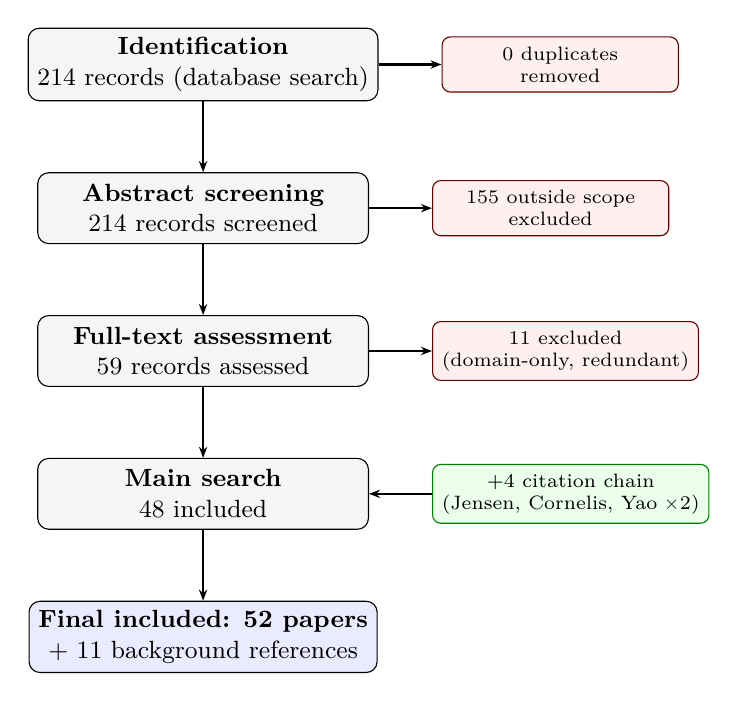
\begin{tikzpicture}[
  box/.style = {draw, rounded corners=4pt, minimum width=4.2cm,
                minimum height=0.9cm, align=center, font=\small,
                fill=gray!8},
  excl/.style = {draw, rounded corners=3pt, minimum width=3.0cm,
                 minimum height=0.7cm, align=center, font=\scriptsize,
                 fill=red!6, draw=red!40!black},
  add/.style  = {draw, rounded corners=3pt, minimum width=3.0cm,
                 minimum height=0.7cm, align=center, font=\scriptsize,
                 fill=green!8, draw=green!50!black},
  arr/.style  = {-{Stealth[length=4pt]}, thick},
]

\node[box] (id) at (0,0) {\textbf{Identification}\\214 records (database search)};
\node[excl, right=0.8cm of id] (dup) {0 duplicates\\removed};
\draw[arr] (id) -- (dup);

\node[box, below=0.9cm of id] (scr) {\textbf{Abstract screening}\\214 records screened};
\node[excl, right=0.8cm of scr] (e1) {155 outside scope\\excluded};
\draw[arr] (id) -- (scr);
\draw[arr] (scr) -- (e1);

\node[box, below=0.9cm of scr] (ft) {\textbf{Full-text assessment}\\59 records assessed};
\node[excl, right=0.8cm of ft] (e2) {11 excluded\\(domain-only, redundant)};
\draw[arr] (scr) -- (ft);
\draw[arr] (ft) -- (e2);

\node[box, below=0.9cm of ft] (main) {\textbf{Main search}\\48 included};
\node[add, right=0.8cm of main] (cit) {+4 citation chain\\(Jensen, Cornelis, Yao $\times$2)};
\draw[arr] (ft) -- (main);
\draw[arr] (cit) -- (main);

\node[box, below=0.9cm of main, fill=blue!8]
  (final) {\textbf{Final included: 52 papers}\\+ 11 background references};
\draw[arr] (main) -- (final);

\end{tikzpicture}
\caption{PRISMA-adapted flow diagram.  Records were retrieved from
scholarly databases; supplementary forward-citation checks on
Google Scholar and Semantic Scholar.  Scopus and Web of Science were not
searched (Section~\ref{sec:limitations}).}
\label{fig:prisma}
\end{figure}

After deduplication, 214 unique records were identified.
Abstract screening removed 155 records outside scope, leaving 59 eligible.
Full-text assessment of these 59 records excluded 11 as outside scope
(domain-only applications, redundant companion papers), yielding 48 records
for inclusion from the main search.  Backward and forward citation-chain
checks on high-citation anchor papers identified 4 additional papers
(Jensen~\&~Shen~2007, Cornelis et~al.~2010, Yao~2010, Yao~2016) that met
all inclusion criteria, bringing the total to 52 included papers.
A further 11 references were retained as background or foundational
(TDA stability theorems, Cover~\&~Hart~1967, survey references).
The final included set of 52 papers is recorded in
\texttt{literature\_log.csv} (released with this paper).

\subsection*{Data extraction}
Each included paper was coded in \texttt{literature\_log.csv} with fields:
paper identifier, first author, year, venue, SJR quartile, citation count,
thematic axis (1/2a/2b/3/4/5), relevance level (core/peripheral/background),
failure-pattern tag (A/B/C/none), read level (abstract/full), key claim,
key finding, and notes.  The \texttt{read\_level} field records the depth of
data extraction (abstract-level coding vs.\ full-text analysis of methods and
results); the ``full-text assessment'' in the PRISMA flow above refers to the
inclusion/exclusion screening step, not the coding depth.  All 52 included
papers were read at full-text depth for the screening decision; data
extraction relied on abstract and methods sections for most papers, with full
experimental re-analysis limited to the ten papers directly involved in the
failure-pattern evidence (Sections~\ref{sec:failure}--\ref{sec:methodology}).
Failure-pattern tagging: A = reduces to known granular
quantity; B = dominance of label-orthogonal geometry; C = self-optimising
evaluation.

\subsection*{Full-text coding of reporting practice}
\label{app:coding}
We coded the reporting practice of 22 papers we were able to read at full
text---13 of them members of the Axis-1 corpus above---released as
\texttt{fulltext\_coding.csv}.  Each row records four presence/absence
fields, judged from the experimental section alone:
\begin{enumerate}[leftmargin=*,itemsep=1pt]
  \item \texttt{all\_features\_baseline} --- does the paper report a
        classification result on the unreduced attribute set, so the reader
        can see whether selection helped?  A mention of the ``original
        dataset'' in a method description does not count; a reported accuracy
        does.
  \item \texttt{reports\_dispersion} --- does at least one results table give
        a standard deviation or per-fold value alongside a mean?
  \item \texttt{significance\_test} --- is a named statistical test
        (Friedman, Wilcoxon, Nemenyi, Bonferroni--Dunn, $t$-test) actually
        carried out on the paper's own results?  Citing a test in related
        work does not count.
  \item \texttt{hyperparam\_ablation} --- does the paper report results at
        more than one value of any hyperparameter of its own method?  Varying
        an external experimental condition, such as an injected noise level,
        does not count.
\end{enumerate}
Every cell carries the quotation or the structural observation it rests on in
the \texttt{evidence} column, so an individual judgement can be checked and
overturned without re-reading the paper.  The fields deliberately record
presence rather than quality: a paper credited with a significance test is
not thereby credited with an appropriate one.  The papers are those we could obtain in full text.
Thirteen of the 22 are members of the Axis-1 corpus above, and constitute 13
of its 25 papers; the remaining nine are from the same literature but outside
our inclusion window.  Section~\ref{sec:significance} therefore reports counts
for both groupings rather than percentages of the field.
Table~\ref{tab:practice_detail} gives the per-paper judgements for the corpus
members.

% AUTO-GENERATED by gen_tables.py -- do not edit by hand.
% Regenerate:  python3 gen_tables.py   Audit:  python3 verify_tables.py
\begin{table}[pos=!htbp]
\caption{Per-paper coding for the 13 Axis-1 corpus papers read at
full text.  B~= all-features baseline; D~= dispersion; S~= significance test;
A~= own-hyperparameter ablation.  $\bullet$~= present, --~= absent.  The
quotation supporting each judgement is in \texttt{fulltext\_coding.csv}.}
\label{tab:practice_detail}
\centering\small
\begin{tabular}{llcccc}
\toprule
Log ID & Paper & B & D & S & A \\
\midrule
T1\_01 & Xia 2020 & -- & -- & -- & -- \\
T1\_02 & Sun 2024 & -- & -- & $\bullet$ & $\bullet$ \\
T1\_03 & Zhang 2025 & $\bullet$ & $\bullet$ & $\bullet$ & -- \\
T1\_04 & Sun 2025 & -- & -- & $\bullet$ & -- \\
T1\_06 & Qian 2024 & -- & -- & $\bullet$ & -- \\
T1\_08 & Ju 2023 & -- & $\bullet$ & -- & -- \\
T1\_09 & Xia 2022 & $\bullet$ & -- & -- & $\bullet$ \\
T1\_10 & Xia 2023 & $\bullet$ & -- & -- & -- \\
T1\_11 & Yang 2024 & -- & -- & $\bullet$ & -- \\
T1\_13 & Xie 2024 & -- & -- & -- & -- \\
T1\_17 & Chen 2021 & -- & -- & $\bullet$ & -- \\
T1\_18 & Peng 2022 & -- & -- & -- & -- \\
T1\_20 & Xia 2024 & -- & -- & $\bullet$ & $\bullet$ \\
\bottomrule
\end{tabular}
\end{table}



\printcredits

\bibliographystyle{cas-model2-names}
\bibliography{refs}

\end{document}
